\documentclass[a4print,english,lof,lot]{univpmphdthesis}
\errorcontextlines=9

\RequirePackage[utf8]{inputenc}
\RequirePackage[T1]{fontenc}

\usepackage{lmodern}
\usepackage[cmex10]{amsmath}
\usepackage{amssymb}
\usepackage{subcaption}
\usepackage{multirow}
\usepackage{booktabs}
\usepackage{framed}
\usepackage{algorithm,algpseudocode}
\usepackage{pgfplots,pgfplotstable}
\usetikzlibrary{pgfplots.groupplots}
\usepackage{tabularx}

\usepackage{tikz}
\usetikzlibrary{shapes,arrows}

\usepackage{tkz-kiviat,numprint}
\usetikzlibrary{decorations.pathreplacing, arrows, fit}
\usepackage{hyperref}


\usetikzlibrary{shadows,arrows,fit,shapes,positioning,calc,backgrounds,spy,decorations.markings}
\usetikzlibrary{backgrounds}

\pgfdeclarelayer{background}
\pgfdeclarelayer{foreground}
\pgfsetlayers{background,main,foreground}

\tikzstyle{bk} = [draw, fill=blue!30, text centered, minimum height=2em, text width=7em, minimum width=6em, minimum height=3em, rounded corners, drop shadow]
\tikzstyle{bkFull} = [draw, fill=blue!30, text centered, minimum height=2em, text width=15em, minimum width=20em, minimum height=3em, rounded corners, drop shadow]
\tikzstyle{bkDec} = [draw, fill=red!40, text centered, minimum height=2em, text width=15em, minimum width=15em, minimum height=3em, rounded corners, drop shadow]
\tikzstyle{cy} = [draw, fill=gray!30, text centered, minimum height=3em, text width=7em, minimum width=2em, cylinder, shape border rotate=90, shape aspect=0.1, drop shadow]
\tikzstyle{cyFull} = [draw, fill=gray!30, text centered, minimum height=3em, text width=7em, minimum width=20em, cylinder, shape border rotate=90, shape aspect=0.1, drop shadow, dashed]
\tikzstyle{bg}=[rectangle,fill=gray!30,inner sep=0.2cm,rounded corners,draw=black!50, dashed]
\tikzstyle{input} = [coordinate]

\tikzset{
	myarrow/.style={
		draw,thick,
		single arrow,
		%text width=1cm,
		minimum height=1cm,
		%anchor=west,
		%fill=white
	},
}

\tikzstyle{vecArrow} = [thick, decoration={markings,mark=at position 1 with {\arrow[semithick]{open triangle 60}}},
double distance=1.4pt, shorten >= 5.5pt, preaction = {decorate}, postaction = {draw,line width=1.4pt, white,shorten >= 4.5pt}]

\tikzstyle{innerWhite} = [semithick, white,line width=1.6pt, shorten >= 4.5pt]




\newcommand{\LegendBox}[3][]{%
	\xdef\fitbox{}%
	\coordinate[#1] (LegendBox_anchor) at (#2) ;
	\foreach \col/\item [count=\hi from 0] in {#3} {
		\node[color = \col,draw,thick,
		fill  = \col,
		minimum width  = 5 ex,
		minimum height = 1 ex,
		name=b\hi,
		] at ([yshift=0 ex,xshift=\hi*40 ex]LegendBox_anchor) {};
		\node[anchor=west,xshift=0.1 ex] at (b\hi.east) (c\hi) {\item};
		\xdef\fitbox{\fitbox(c\hi)}
	}%
	\node [fit=\fitbox(LegendBox_anchor), minimum width = 0 ex] {};
}


\newcommand{\chref}[1]{Chapter~\ref{#1}}
\newcommand{\secref}[1]{Section~\ref{#1}}
\newcommand{\subsecref}[1]{Subsection~\ref{#1}}
\newcommand{\apxref}[1]{Appendix~\ref{#1}}

\newcommand{\figref}[1]{\figurename~\ref{#1}}
\newcommand{\tableref}[1]{Table~\ref{#1}}

\newcommand*\rfrac[2]{{}^{#1}\!/_{#2}}


\def\N{{\mathbb{N}}}
\def\Z{{\mathbb{Z}}}
\def\R{{\mathbb{R}}}

%%%%%%%%%%%%%%%%%%%%%%%%%%%%%%%%%%%%%%%%%%%%%%%%%%%%%%%%%%%
% Metadata
%%%%%%%%%%%%%%%%%%%%%%%%%%%%%%%%%%%%%%%%%%%%%%%%%%%%%%%%%%%
\phdschool{Scuola di Dottorato di Ricerca in Scienze dell'Ingegneria}
\phdfaculty{Facolt\`{a} di Ingegneria}
\phdcurriculum{Curriculum in Ingegneria Elettronica, Elettrotecnica e delle Telecomunicazioni}
\phdtitle{Deep Learning for Sound Event Detection and Classification}
%\phdsubtitle{con questa bellissima classe} % NON NECESSARIO
\phdauthor{Fabio Vesperini}
\phdadvisor{Prof.~Stefano Squartini}
%\phdcoadvisor{Prof.~Michele Blu} % IN TEORIA NON E' AMMESSO
\phdcurriculumadvisor{Prof.~Francesco Piazza}
\phdcycle{17}
\thesisdedication{alla mia famiglia}
\phdlocation{Ancona}
\phdtime{Ottobre 2018}
%%%%%%%%%%%%%%%%%%%%%%%%%%%%%%%%%%%%%%%%%%%%%%%%%%%%%%%%%%%

% Solo per generare testo...
\usepackage{lipsum}

\begin{document}

%%%%%%%%%%%%%%%%%%%%%%%%%%%%%%%%%%%%%%%%%%%%%%%%%%%%%%%%%%%
% Front matter contents
%%%%%%%%%%%%%%%%%%%%%%%%%%%%%%%%%%%%%%%%%%%%%%%%%%%%%%%%%%%
\frontmatter

\maketitle

%\begin{thesisacknowledge}
%\lipsum[1-2]
%\end{thesisacknowledge}

%\begin{thesisacknowledge}[italian]
%\lipsum[1-2]
%\end{thesisacknowledge}

\begin{thesisabstract}
\lipsum[1-3]
\end{thesisabstract}

\thesistoc

%%%%%%%%%%%%%%%%%%%%%%%%%%%%%%%%%%%%%%%%%%%%%%%%%%%%%%%%%%%
% Main matter contents
%%%%%%%%%%%%%%%%%%%%%%%%%%%%%%%%%%%%%%%%%%%%%%%%%%%%%%%%%%%
\mainmatter

\chapter{Introduction}\label{ch:intro}

Human cognition relies on the ability to sense, process, and understand the surrounding environment and its sounds.
Although the skill of listening and understanding their origin is so natural for living beings, it still results in a very challenging task for computers. In recent years several novel methods have been proposed to analyze this information automatically, and several new applications have emerged \cite{virtanen2018computational}. However, the creation of ``machine listening'' algorithms that can mimic this cognitive feature by means of artificial systems remains a very challenging task. 

Automatic sound event detection (SED), also known as acoustic event detection, is nowadays considered as one of the most important topics in the field of computational auditory scene analysis (CASA). Thanks to works like Bregman's ``Auditory Scene Analysis: The Perceptual Organization of Sound''~\cite{bregman1994auditory}, we can trace back the birth of this field to 1994, when the field of auditory scene analysis (ASA) was introduced in order to model humans' sound perception. Following this work, many other contributions were written aiming to describe how artificial systems can be designed in order to perceive sounds similarly to as humans do; most of these works will be later collected in Divenyi's book~\cite{divenyi2004speech} in 2004.

Nowdays, one of the main subject of interest in technological research regards systems deployed for surveillance applications. Surveillance can be seen as control of public safety or as the supervision of private environments where people may live alone. 
In fact, the increasing level of public security over the past decades has motivated the installation of sensors such as cameras or microphones in public places (stores, subway, airports, etc.), while is possible to effectively consider personal multimedia devices (smartphones, tablets, etc.) as virtual assistant which is able to monitor the user and eventually intervene in case of necessity without having the need for a physical interface (i.e., keyboard) anymore.
Thus, the need of unsupervised situation assessment stimulated the signal processing community towards experimenting with several automated frameworks, due to their potential in several engineering applications.

In these contexts, sound or sound sensing can be advantageous with respect to other modalities of multimedia processing.  
This is the case of acoustic surveillance \cite{crocco2016audio}, healthcare monitoring \cite{peng2009healthcare, foggia2015reliable} or urban sound analysis \cite{salamon2017deep}, where the short duration of certain events (i.e., a human fall, a gunshot or a glass breaking) or the personal privacy motivate the exploitation of the audio information rather than, e.g., the image processing. 
In addition, audio processing is often less computationally demanding compared to other multimedia domains, thus embedded devices can be easily equipped with microphones and sufficient computational capacity to locally process the signal captured. 
These could be smart home devices for home automation purposes or sensors for wildlife and biodiversity monitoring (i.e., bird calls detection \cite{grill2017two}). 
Some of these applications have already become commercial products that are able recognize certain specific sound categories in realistic environments and improve home security \cite{audioanalytic}  or companies with as much impactful missions, such as preserve the Rainforest from illegal deforestation \cite{rainforest}.

The type of information to be extracted with these algorithms depends on the application. In particular, we can sort the sound analysis tasks explored in this work into two high-level categories: sound event \textit{detection} and sound event \textit{classification}.
In sound event detection (SED), or acoustic event detection, the goal is to detect the onset and offset times for a variety of sound events captured in an audio recording. 

In sound event classification, the goal is to categorize an audio recording into one of a set of predefined categories by associating a textual descriptor.

In controlled laboratory conditions where the data used to develop computational sound scene and event analysis methods matches well with the test data, it is possible to achieve relatively high accuracies in the detection and classification of sounds.  However, there are several complexities in computational sound analysis and current technologies face many challenges, mainly related to the acoustics of sound scenes and events, when they are employed in realistic environments.
Among these challenges we can include:
\begin{itemize}
	\item the effect of the environment acoustics: reverberation, background noises and the channel coupling (impulse response) between the source and the recording equipment;
	\item the intra-class variability, i.e., high difference of the acoustic characteristics of even a single class of sounds and on the other hand the similarity of many different types of sounds to the target events  \cite{stowell2015acoustic};
	\item the \textit{polyphony}, i.e. the occurrence of multiple simultaneous events. In realistic environments there
are almost always multiple sources producing sound at the same time. 
\end{itemize}

In addition to these complications related to the acoustics of sound scenes and
events, there are also several fundamental limitations related to the computational methods. In particular, to develop effective models based on the \textit{deep learning} paradigm, a very large set of examples of the
target (and non-target) sounds is required. In contrast to the situation in image classification,
 currently available datasets that can be used to train such systems are more limited in size, diversity, and number of event
 instances, even though recent contributions such as AudioSet \cite{gemmeke2017audio} or the DCASE challenges
and related workshops \cite{DCASE2017Workshop, mesaros2016tut, dcase2018web} have provided public available datasets to reduce this gap.



\section{The Deep Learning Approach for Sound Event Detection and Classification}

\begin{figure}[b]
	\centering
	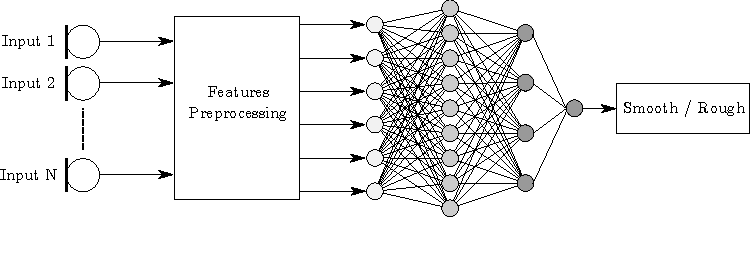
\includegraphics[width=\linewidth]{img/flowchart_1.pdf}
	\caption[Basic structure]{Basic structure of an audio analysis system.}
	\label{fig:base-system}
\end{figure}

\begin{figure}[tb]
	\centering
	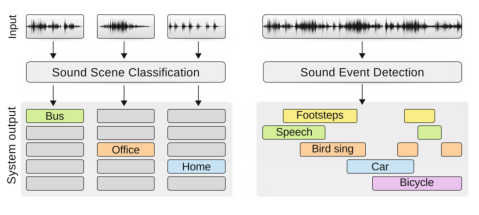
\includegraphics[width=\linewidth]{img/sed_sec.pdf}
	\caption[System input and output ]{System input and output for the two main analysis systems: sound scene classification and sound event detection.}
	\label{fig:system-io}
\end{figure}

The typical computational sound scene
or event analysis system based on machine learning is
depicted in \figref{fig:base-system}, while the different input and output respectively for classification and detection systems
are illustrated in \figref{fig:system-io}.

As the first stage, all the systems take as input one or more audio
signals, either in real-time, captured by a microphone, or offline, from an
audio recording. In this work, we assume always discrete-time signals,
obtained by using analog-to-digital converters. 

The \textit{Feature Extraction} block consists
of different processing stages and outputs acoustic features, as the actual analysis of
audio is rarely based on the raw audio signal, but rather on the compact signal
representation with features. The purpose of the feature extraction is to obtain
information sufficient for detecting or classifying the target sounds, making the
subsequent modeling stage computationally cheaper and also easier to achieve with
limited amount of development material. Very often the feature extraction procedure is also preceded by the down-mixing the audio signal into a single (mono) channel and re-sampling it into fixed sampling frequency.
Although every application could require a specific set of features able to highlight the discriminating particularities of each data sample, the most common representations used
for audio signals are non-linear representation for magnitudes (power spectra and logarithm) and nonlinear frequency scaling (mel-frequency scaling). 
More details of the acoustic features extraction process for each examined case-study will be provided in further chapters.


The \textit{Deep Learning}-based model takes the acoustic features as input and it is trained to produce an output which will assign a class label depending on the application. Almost all the system presented in this work are based on the supervised machine learning approach, where the system is trained using labeled examples of sounds from each of target sound type. 
At the development stage, the obtained acoustic features are used together with
reference annotations of the audio training examples, to learn models for the
sound classes of interest. Annotations contain information about the presence of
target sound classes in the training data, and are used as a reference information
to automatically learn a mapping between acoustic features and class labels. The
mapping is represented by acoustic models. The learning process consists in updating the parameters or \textit{weights} of the neural network, searching for the optimal model that minimize a certain cost-function. 
At the usage stage, the learned acoustic models are used to do recognition (detection or classification), which predicts labels
for the input audio. The recognition stage may also involve temporal models and
post-processing of labels.


After a prediction is obtained through the trained acoustic model, the \textit{Post Processing} stage translates this signal into the effective activity information for each class. Very often this relies on a simple \textit{thresholding} operation or on the selection of the most probable class.


\section{State of the Art}

Traditionally, the computational acoustic event analysis has been approached with statistical modelling methods, including Hidden Markov Models (HMM) \cite{degara2011onset}, Gaussian Mixture Models (GMM) \cite{heittola2010audio}, Non-negative Matrix Factorization (NMF) \cite{carabias2011musical} and support vector machines (SVM) \cite{guo2003content}. 

In the recent era of the ``Deep Learning'', different neural network architectures have been successfully used for sound event detection and classification tasks, including feed-forward neural networks (FNN) \cite{mcloughlin2015robust}, deep belief networks \cite{mohamed2012acoustic}, convolutional neural networks (CNNs) \cite{piczak2015environmental} and Recurrent Neural Networks (RNNs) \cite{graves2013speech}. In addition, these architectures laid the foundation for end-to-end systems \cite{trigeorgis2016adieu, wu2017end}, in which the feature representation of the audio input is automatically learnt from the raw audio signal waveforms. 

The use of deep learning models has been motivated by the increased availability of datasets and computational resources and resulted in significant performance improvements, outperforming in most of the cases the human accuracy \cite{sailor2017unsupervised}.
The methods based on CNNs and RNNs have established the new state-of-the-art performance on the sound event detection task (SED), thanks to the capabilities to learn the non-linear relationship between time-frequency features of the audio signal and a target vector representing sound events. In \cite{espi2015}, the authors show how ``local'' patterns can be learned by a CNN and can be exploited to improve the performance of detection and classification of non-speech acoustic events occurring in conversation scenes, in particular compared to a FNN-based system which processes multiple resolution spectrograms in parallel. 

This success is a result of close academic-industrial collaboration, which started from the speech or speaker recognition task and extended to the analysis of non-speech, music and sound scenes and events. The combination of the CNN structure with recurrent units has increased the detection performance by taking advantage of the characteristics of each architecture. This is the case of convolutional recurrent neural networks (CRNNs) \cite{cakir2017convolutional}, which provided state-of-the-art performance especially in the case of polyphonic SED. CRNNs consolidate the CNN property of local shift invariance with the capability to model short and long term temporal dependencies provided by the RNN layers. This architecture has been also employed in almost all of the most performing algorithms proposed in the last editions of research challenges such as the IEEE Audio and Acoustic Signal Processing (AASP) Challenge on  Detection and Classification of Acoustic Scenes and Events (DCASE) \cite{DCASE2017Workshop}. 

On the other hand, if the datasets are not sufficiently large, problems such as overfitting can be encountered with these models, which typically are composed of a considerable number of free-parameters (i.e., more than 1M). 

Encouraging polyphonic SED performance have been obtained using CapsNets in preliminary experiments conducted on the Bird Audio Detection task in occasion of the DCASE 2018 challenge \cite{vesperini2018capsule}, confirmed by the results reported in \cite{iqbal2018capsule}.
The CapsNet \cite{sabour2017dynamic} is a recently proposed architecture for image classification and it is based on the grouping of activation units into novel structures introduced in \cite{hinton2011transforming}, named \textit{capsules}, along with a procedure called dynamic routing. The capsule has been designed to represent a set of properties for an entity of interest, while dynamic routing is included to allow the network to implicitly learn global coherence and to identify part-whole relationships between capsules.


%TODO EXTEND SoA ?
%Labels extracted with a SED system usually allow us to achieve a better insight of the considered acoustic scenario, for example they can be used as mid-level representation useful for other CASA research areas. In~\cite{chu2009environmental, heittola2010audio}, for example, authors make use of SED for designing audio context recognition systems, while in~\cite{shah2012lifelogging} and~\cite{wichern2010segmentation} SED is exploited for automatic tagging and audio segmentation respectively. Moreover, SED also found many direct applications in a variety of scenarios, some examples being context-based indexing and retrieval in multimedia databases~\cite{xu2008audio}, unobtrusive health monitoring~\cite{peng2009healthcare}, and audio-based surveillance~\cite{harma2005automatic, crocco2014surveillance, Principi2016a}.
%As we can notice from~\cite{heittola2010audio, peng2009healthcare}, hidden Markov models (HMMs) have been widely used in the literature with the purpose of modelling acoustic events in a SED system, usually in terms of a Gaussian mixture model (GMM). In recent years, new approaches to SED have been proposed, marking a distinct trend towards the use of artificial neural networks (ANNs)-based systems. An interesting comparison between computational costs of different systems is carried out in~\cite{sigtia2016automatic} highlighting that ANNs are able to achieve top performance at the cost of being the most computationally expensive approach. A brilliant example of such performance is given in~\cite{hershey2016cnn}, where different ANNs are trained on a big video dataset and then used for different scopes, among which also SED. For a wider overview of the most recent and powerful SED techniques the reader can refer to the comprehensive analysis carried out by Sharan \emph{et al.}\ in~\cite{sharan2016overview}.

%%%%%%%%%%%%%%%%%%%%%%%%%%%%%%%%%%%%%%%%%%%%%%%%%%%%%%%%%%%%%%%%%%%%%


%The use of deep learning models has been motivated by the increased availability of datasets and computational resources and resulted in significant performance improvements.
%The methods based on CNNs and RNNs have established the new state-of-the-art performance on the SED task, thanks to the capabilities to learn the non-linear relationship between time-frequency features of the audio signal and a target vector representing sound events. In \cite{espi2015}, the authors show how ``local'' patterns can be learned by a CNN and can be exploited to improve the performance of detection and classification of non-speech acoustic events occurring in conversation scenes, in particular compared to a FNN-based system which processes multiple resolution spectrograms in parallel. 

%The combination of the CNN structure with recurrent units has increased the detection performance by taking advantage of the characteristics of each architecture. This is the case of convolutional recurrent neural networks (CRNNs) \cite{cakir2017convolutional}, which provided state-of-the-art performance especially in the case of polyphonic SED. CRNNs consolidate the CNN property of local shift invariance with the capability to model short and long term temporal dependencies provided by the RNN layers. This architecture has been also employed in almost all of the most performing algorithms proposed in the recent editions of research challenges such as the DCASE \cite{DCASE2017Workshop}. On the other hand, if the datasets are not sufficiently large, problems such as overfitting can be encountered with these models, which typically are composed of a considerable number of free-parameters (i.e., more than 1M). 



\section{Case studies}
In this work, different application of deep learning for computational audio models in real environments are analyzed. They are evaluated and compared with state-of-the-art methods on different databases, some of these resulting novel approaches. The broad and extensive experimental evaluations highlight the advantages provided by the acoustic models based on deep learning.

The addressed tasks are the following:
\begin{itemize}
	\item Sound event \textit{Classification}:
	\begin{itemize}
		\item Snore sounds excitation localization;
		\item Acoustic road surface roughness classification;
		\item Bird audio detection;
	\end{itemize}
	\item Sound event \textit{Detection}:
	\begin{itemize}
		\item Overnight snore sound detection;
		\item Rare sound event detection;
		\item Voice activity detection in multiroom environments;
	\end{itemize}
	\item \textit{Polyphonic} Sound event Detection:
	\begin{itemize}
		\item A neural network approach for sound event detection in real life audio;
		\item Polyphonic sound event detection by using CapsNets		
	\end{itemize}
\end{itemize}






\graphicspath{{2_background/}}
\chapter{Background}\label{ch:backg}

The Computers are able to perform complex calculus operations in a short amount of time.
However computers cannot compete with humans in dealing with: common sense, ability to recognize people, objects, sounds, comprehension of natural language, ability to learn, categorize, generalize.

Therefore, why does the human brain show to be superior w.r.t common computers for these kind of problems?
Is there any chance to mimic the mechanisms characterizing the way of working of our brain in order to produce more efficient machines?

In the field of signal analysis, the aim is the characterization of such real-world signals in terms of \textit{signal models}, which can provide the basis for a theoretical description of a signal processing system. They are potentially capable of letting us learn a great deal about the signal source, without having to have the source available.

The ``Deep Learning'' is a new area of machine learning
research, which has been introduced with the objective of moving
Machine Learning closer to one of its original goals: Artificial Intelligence. Deep Learning is about learning multiple levels of
representation and abstraction that help to make sense of data
such as images, sound, and text.

Therefore, in this chapter a theoretical description of the principal Deep Neural Network (DNN) architectures is given. In addition, the algorithms used for their parameter estimation are described, with a focus on the most widely model structure used in the field of the computational acoustic event analysis.


\subsection{Deep Neural Network architectures for for Analysis of Sound Scenes and Events}

%\textbf{ndRob} to complete, 3 pages with figures
%\begin{itemize}
%\item formula (notazione matriciale) del calcolo output di ogni rete
%\end{itemize}

A \textit{biological Neural Networks} is a big set of specialized cells (\textit{neurons}) connected among them, which memorize and process information, thus controlling the body activities they belong to.

\begin{figure}[t]
\centering
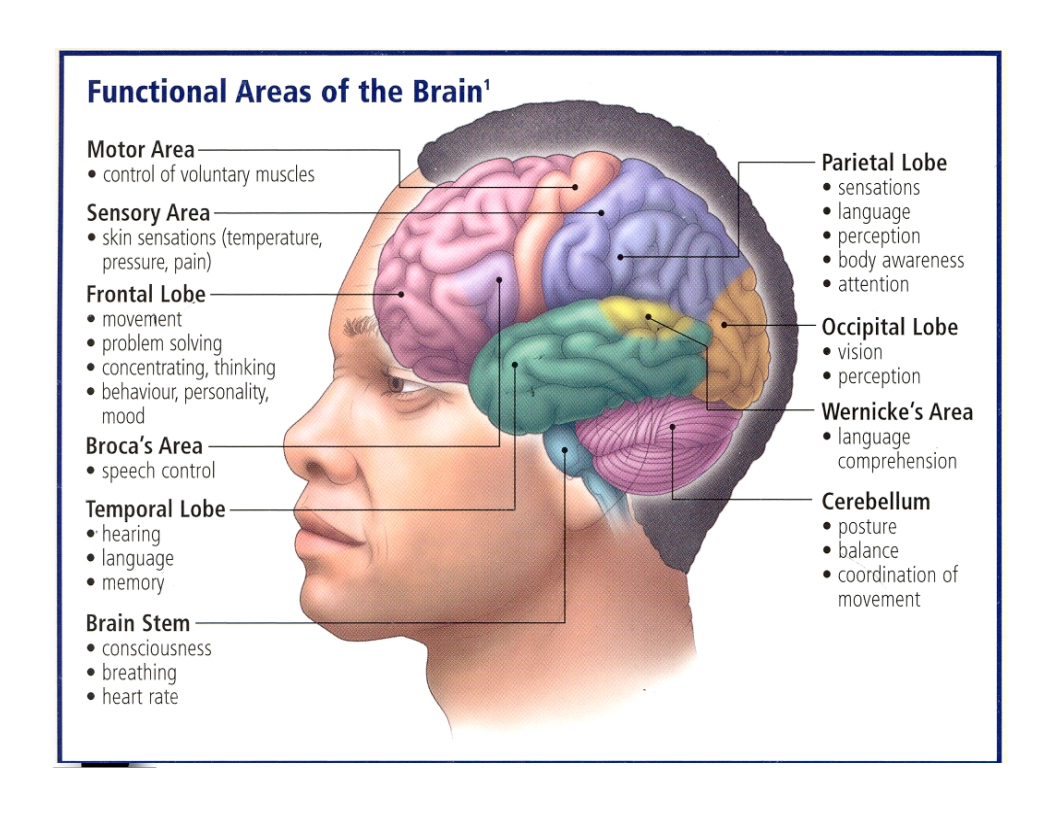
\includegraphics[width=0.65\linewidth]{img/Brain}
\caption{The human brain.}
%\label{vv}
\end{figure}

The \textit{neuron} model is composed of:
\begin{itemize}
\item DENDRITE: input terminal
\item CELL BODY (Nucleus): processing core
\item AXON: output way-out
\item SYNAPSES: output terminal (with weight)
\end{itemize}

%The Biological neurons are electro-chemical devices, operating at low rates ($\approx mses$).
%Digital circuits operate at very high rates ($\approx nsec$).

\begin{figure}[t]
\centering
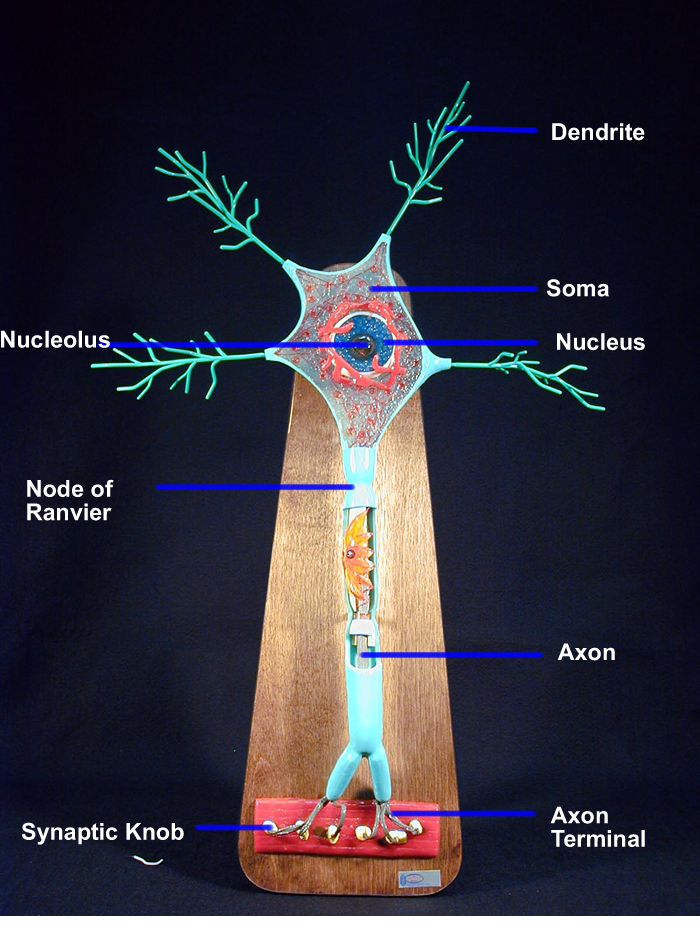
\includegraphics[width=0.4\linewidth]{img/neuron_model}
\caption{The neuron model.}
%\label{aa}
\end{figure}

The \textit{neuron} properties can be described in:
\begin{itemize}
\item LOCAL SIMPLICITY: the neuron receives stimuli (excitation or inhibition) from dendrites and produces an impulse to the axon which is proportional to the weighted sum of the inputs;
\item GLOBAL COMPLEXITY: the human brain possess 
$\mathcal{O}(10^{10})$ 
neurons, with more than 10K connections each;
\item LEARNING: even though the network topology is relatively fixed, the strength of connections (synaptic weights) can change when the network is exposed to external stimuli;
\item DISTRIBUTED CONTROL: no centralized control, each neuron reacts only to its own stimuli;
\item TOLERANCE TO FAILURES: performance slowly decrease with the increase of failures.
\end{itemize}

The biological Neural Networks are able to solve very complex tasks in few time instants (like memorization, recognition, association, and so on.)

\begin{figure}[t]
\centering
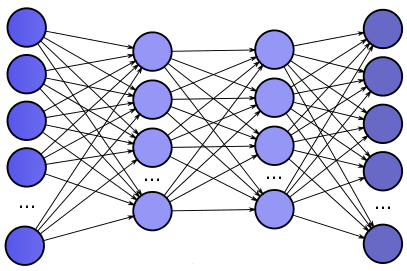
\includegraphics[width=0.4\textwidth]{img/ANN}
\caption{The Artificial Neural Network.}
%\label{aa}
\end{figure}

The \textit{Artificial Neural Networks} (ANNs) are defined as \textit{Massively parallel distributed processors made up of simple processing units having a natural propensity for storing experiential knowledge and making it available for use} (Haykin, 2008).

An ANN resembles the brain in two aspects:
\begin{enumerate}
\item Knowledge is acquired by the network from its environment through a learning process;
\item Synaptic weights are used to store the acquired knowledge.
\end{enumerate}

A \textit{neuron} is an information-processing unit that is fundamental to the operation of a neural network.
The model of a neuron is composed of three basic elements of the neural model:
\begin{itemize}
\item a \textit{set of synapses}, or connecting links, each of which is characterized by a weight or strength of its own, $w_{kj}$;
\item an \textit{adder} for summing the input signals, weighted by the respective synaptic strengths of the neuron; the operations described here constitute a linear combiner;
\item an \textit{activation function} for limiting the amplitude of the output of a neuron. Typically, the normalized amplitude range of the output of a neuron is written as the closed unit interval [0,1], or, alternatively, [-1,1].
\end{itemize}
The neural model also includes an externally applied \textit{bias}, denoted by $b_k$.

\begin{figure}[t]
\centering
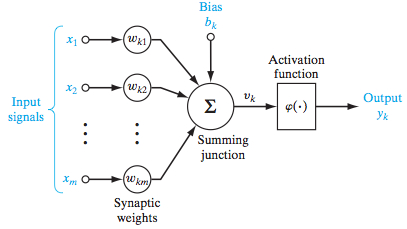
\includegraphics[width=0.8\linewidth]{img/NeuronModel.jpg}
%\label{aa}
\caption{The artificial neuron model.}
\end{figure}

Therefore, the mathematical description of neuron activity can be defined as:
\begin{eqnarray}
{ u }_{ k }=\sum _{ j=1 }^{ m }{ { w }_{ kj } } { x }_{ j }\\ 
{ y }_{ k }=\varphi \left( { u }_{ k }+b_{ k } \right)
\end{eqnarray}
where:
\begin{itemize}
\item ${ x }_{ 1 },{ x }_{ 2 },\cdots ,{ x }_{ m }$ are the input signals;
\item ${ w }_{ k1 },{ w }_{ k2 },\cdots ,{ w }_{ km }$ are the respective synaptic weights of neuron $k$;
\item $u_k$ is the linear combiner output due to the input signals;
\item $b_k$ is the bias;
\item $\varphi(\cdot)$ is the activation function;
\item $y_k$ is the output signal of the neuron.
\end{itemize}

The types of \textit{activation non-linear functions} $\varphi(x)$ are:
\begin{itemize}

\item the \textit{threshold function}: in engineering, this form of a threshold function is commonly referred to as a Heaviside function;
\begin{eqnarray}
\varphi \left( v \right) =1\quad if\quad v\ge 0 \\ 
\varphi \left( v \right) =0\quad if\quad v<0
\end{eqnarray}
\begin{figure}
\centering
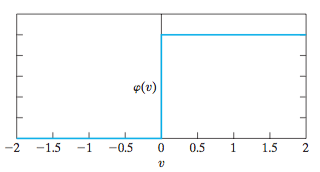
\includegraphics[width=0.4\textwidth]{img/Heaviside}
\caption{The threshold non-linear function.}
%\label{aa}
\end{figure}

\item the \textit{sigmoid function}: it is defined as a strictly increasing function that exhibits a graceful balance between linear and nonlinear behavior; an example of the sigmoid function is the \textit{logistic function} defined by:
\begin{equation}
\varphi \left( v \right) =\frac { 1 }{ 1+exp\left( -av \right)  } 
\end{equation}
\begin{figure}
\centering
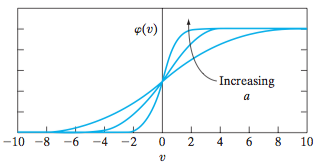
\includegraphics[width=0.4\textwidth]{img/sigmoid}
\caption{The sigmoid non-linear function.}
%\label{aa}
\end{figure}

\item the \textit{ hyperbolic tangent } ($tanh$): it is simply a scaled and shifted version of the sigmoid function:
\begin{equation}
\varphi(x) = \frac{1-e^{-2x}}{1+e^{-2x}}
\end{equation}
\begin{figure}[t]
\centering
	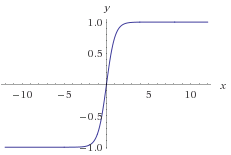
\includegraphics[width=0.4\textwidth]{img/tanh}
	\caption{The $tanh$ non-linear function.}
%				\label{aa}
\end{figure}

\item the \textit{ Rectifier Linear Unit} ($ReLU$):
\begin{equation}
\varphi(x) = \text{max}(0,x)
\end{equation}
\begin{figure}[t]
\centering
	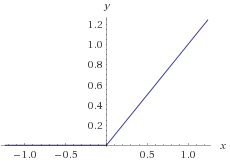
\includegraphics[width=0.4\textwidth]{img/relu}
	\caption{The $ReLU$ non-linear function.}
%				\label{ee}
\end{figure}

\item the $softmax$: it is used on the last layer of a classifier setup: the outputs of the softmax layer represent the probabilities that a sample belongs to the different classes. Indeed, the sum of all the output is equal to $1$.
			%In this case the targets are \textit{one-hot} vectors and the cost-function is the \textit{categorical cross-entropy}.
\begin{equation}
\varphi(x_k) = \frac{e^{x_k}}{\sum_{j=1}^{N}e^{x_j}} \text{ for }  k=1,\dots,K
\end{equation}
\begin{figure}[t]
\centering
	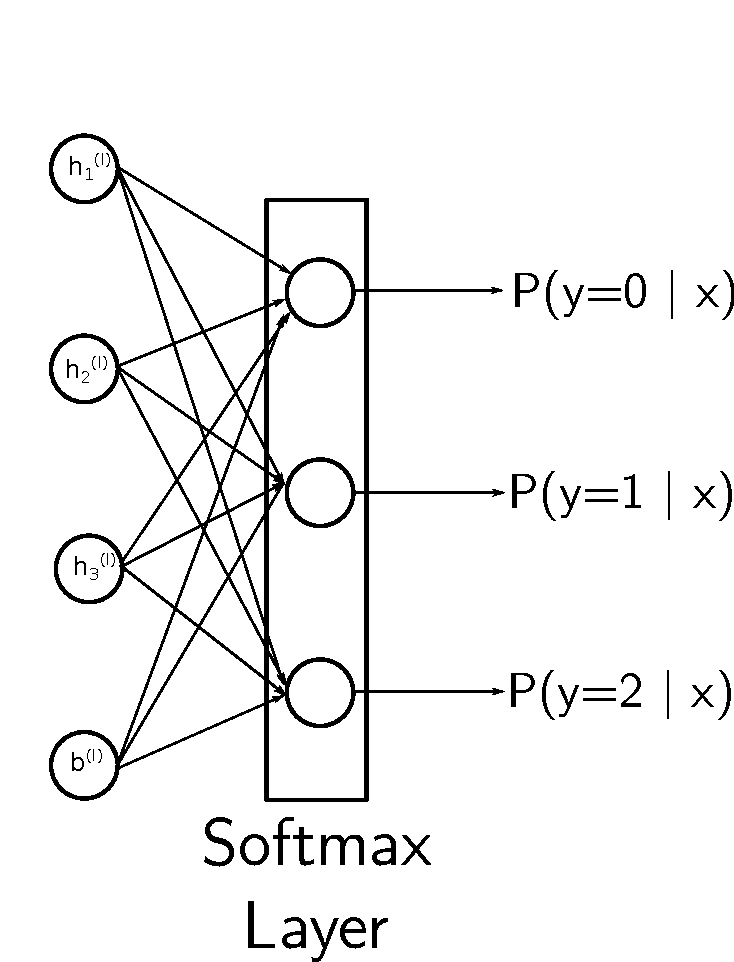
\includegraphics[width=0.4\textwidth]{img/softmax}
	\caption{The $\textit{softmax}$ layer in a neural network classifier.}
%					\label{aa}
\end{figure}	
			
%			\item $\mathbf{maxout}$ - the output is the maximum value among $K$ linear models applied to a given input (or an hidden activation): $\varphi(x_k) = \max(x_k)$ with $k=1,\dots,K$.\\
%			It is supposed to be combined with dropout.
			
	%		It is an approximate model averaging technique. A single maxout unit performs a piecewise linear approximation to an arbitrary convex function. Maxout networks learn not just the relationship between hidden units, but also the activation function of each hidden unit.	
		
				
		
%				\begin{figure}
%				\centering
%					\includegraphics[width=0.75\textwidth]{img/maxout}
%					\caption{Example of an MLP with $\mathbf{maxout}$ units. Picture courtesy of GoodFellow et al. 2013}
%%					\label{rr}
%				\end{figure}

\end{itemize}

% ****************************************************+
%NEURAL NETWORKS VIEWED AS DIRECTED GRAPHS
%
%A neural network is a \textbf{directed graph} consisting of nodes with interconnecting synaptic and activation links and is characterized by four properties:
%
%\begin{enumerate}
%\item Each neuron is represented by a set of linear synaptic links, an externally applied bias, and a possibly nonlinear activation link. The bias is represented by a synaptic link connected to an input fixed at $+1$.
%\item The synaptic links of a neuron weight their respective input signals.
%\item The weighted sum of the input signals defines the induced local field of the neuron in question
%\item The activation link squashes the induced local field of the neuron to produce an output
%\end{enumerate}
%
%\begin{figure}
%\centering
%\includegraphics[width=0.55\textwidth]{img/NeuronGraph.jpg}
%\caption{The Neuron graph model.}
%%\label{key}
%\end{figure}
%
%When the focus of attention is restricted to signal flow from neuron to neuron, we may use a reduced form of this graph by omitting the details of signal flow inside the individual neurons. Such a directed graph is said to be \textit{partially complete}. It is characterized as follows:
%
%\begin{enumerate}
%\item Source nodes supply input signals to the graph.
%\item Each neuron is represented by a single node called a computation node.
%\item The communication links interconnecting the source and computation nodes of the graph carry no weight; they merely provide directions of signal flow in the graph.
%\end{enumerate}
%
%%\begin{figure}
%%\centering
%%\includegraphics[width=0.55\textwidth]{img/NeuronPGraph.jpg}
%%%\label{aa}
%%\caption{ee}
%%\end{figure}
%
%
%Graphical representations of a neural network
%
%\begin{itemize}
%\item \textbf{Block Diagram} $\rightarrow$ functional description of the network
%\item \textbf{Architectural Graph} $\rightarrow$ description of the network layout
%\item \textbf{Signal-Flow Graph} $\rightarrow$ complete description of the signal flow in the network
%\end{itemize}

% *********************************************************+

The manner in which the neurons of a neural network are structured is intimately linked with the learning algorithm used to train the network. % Therefore, the learning algorithms (rules) used in the design of neural networks as being structured.
There, the \textit{network architectures} (structures) is defined.
In general, two different classes of network architectures are identified:
\begin{enumerate}

%\item \textit{Single-Layer Feedforward Networks} (SLFN):
%
%\begin{itemize}
%\item We have an input layer of source nodes that projects directly onto an output layer of neurons (computation nodes), but not vice-versa 
%\item Such a network is called a single-layer network, with the designation \emph{single-layer} referring to the output layer of computation nodes (neurons). 
%\item We do not count the input layer of source nodes because no computation is performed there.
%\end{itemize}
%
%\begin{figure}
%\centering
%\includegraphics[width=0.35\textwidth]{img/SLFN}
%%\label{aa}
%\caption{The Single-Layer Feedforward Network.}
%\end{figure}


\item \textit{Multilayer Feedforward Networks} - (FFNN):

it is characterized by the presence of one or more hidden layers, whose computation nodes are correspondingly called \textit{hidden neurons} (or hidden units);
the term \textit{hidden} refers to the fact that this part of the neural network is not seen directly from either the input or output of the network. 
The function of hidden neurons is to intervene between the external input and the network output in some useful manner. By adding one or more hidden layers, the network is enabled to extract higher-order statistics from its input. 
%\item Example: \textbf{10-4-2 network} $->$ it has 10 source nodes, 4 hidden neurons, and 2 output neurons.


\begin{figure}
\centering
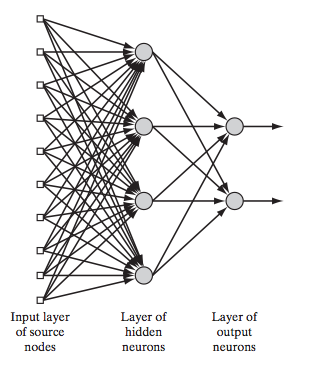
\includegraphics[width=0.4\textwidth]{img/MLP}
%\label{aa}
\caption{The Multilayer Feedforward Network.}
\end{figure}


%\textbf{ndRob} to complete, 1 pages with figure
%\begin{itemize}
%\item struttura a layer
%\item notazione matriciale con indici layer
%\end{itemize}

The MLP is a well known kind of artificial neural network introduced in 1986 \cite{Rumelhart86-LRB}. 
Each node applies an activation function over the weighted sum of its inputs. 
The units are arranged in layers, with feed forward connections from one layer to the next. 
The stochastic gradient descent with error back-propagation algorithm is used for the supervised learning of the network. 
In the forward pass, input examples are fed to the input layer, and the resulting output is propagated via the hidden layers towards the output layer. At the backward pass, the error signal originating at the output neurons is sent back through the layers and the network parameters (i.e., weights and biases) are tuned.

A single neuron can be formally described as:
\begin{equation}
%g(\mathbf{u}[n])=\varphi \left(\left(\begin{matrix} \sum _{ j=1 }^{ D }{w_j u_j[n] }  \end{matrix} \right) + b\right),
g(\mathbf{u}[n])=\varphi \left(\sum _{ j=1 }^{ D }{w_j u_j[n] } + b\right),
\end{equation}
where $\mathbf{u}[n] \in \mathbb{R}^{D\times 1}$, the bias $b$ is an externally applied term and $\varphi(\cdot)$ is the non-linear activation function.
Thus, the mathematical description of a one-hidden-layer MLP is a function $\mathbf{f}:\mathbb{R}^D \rightarrow \mathbb{R}^{D'}$, where $D'$ is the size of the output vector, so:
\begin{equation}
\mathbf{f}(\mathbf{u}[n]) = 	\varphi \left( \mathbf{b}_2 + \mathbf{W}_2 \left( \varphi \left( \mathbf{b}_1 + \mathbf{W}_2 \cdot \mathbf{u}[n]\right) \right) \right),
\end{equation}
where $\mathbf{W}_i$ and $\mathbf{b}_{i}$ are the respective synaptic weights matrix and the bias vector of the $i$-th layer.
The behaviour of this architecture  is  parametrized  by  the connection weights, which are adapted during the supervised network training.



\item \textit{Convolutional Neural Networks}(CNN)

\begin{figure}
	 \centering
	 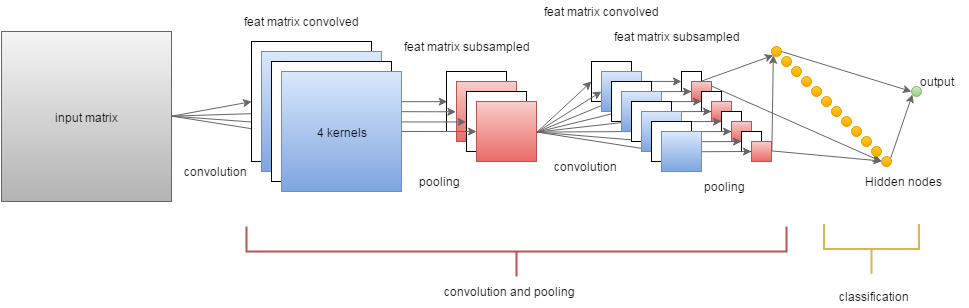
\includegraphics[width=0.9\columnwidth]{img/CNN}
%	 \label{ee}
	 \caption{The Convolutional Neural Network.}
	\end{figure}

%\textbf{ndRob} to complete,  1 pages with figure

Convolutional neural networks are feedforward neural networks similar to multilayer perceptron, with some special layers.

%Matrix convolution: it is performed between a bigger matrix, which is the input, and a smaller matrix, the convolutional kernel.

\begin{figure}[t]
		\centering
		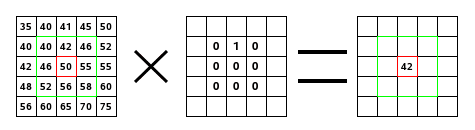
\includegraphics[width=0.7\columnwidth]{img/convolution-calculate}
%		\label{ee}
		\caption{The convolution operation.}
	\end{figure}
	


%	\item Convolution kernels, by training, adapt on recurrent input patterns, becoming themselves similar to those patterns. As a result an activation of the kernel is given when a specific pattern occurs. 
Convolution kernels process the input data matrix by dividing it in \textit{local receptive fields}, a region of the same size of the kernel, and sliding the local receptive field across the entire input.
Each hidden neuron is thus connected to a local receptive field, and all the neurons form a matrix called \textit{feature map}.
%We can have multiple feature maps.
The weights in each \textit{feature map} are \textit{shared}: all hidden neurons are aimed to detect exactly the same pattern just at different locations in the input image. 

The main advantages of this network is the robust pattern recognition system characterized by a strong immunity to pattern shifts.

Pooling layer just reduces the dimension of the matrix by a rule: a submatrix of the input is selected, and the output is the maximum value of this submatrix.
	
	\begin{figure}
		\centering
		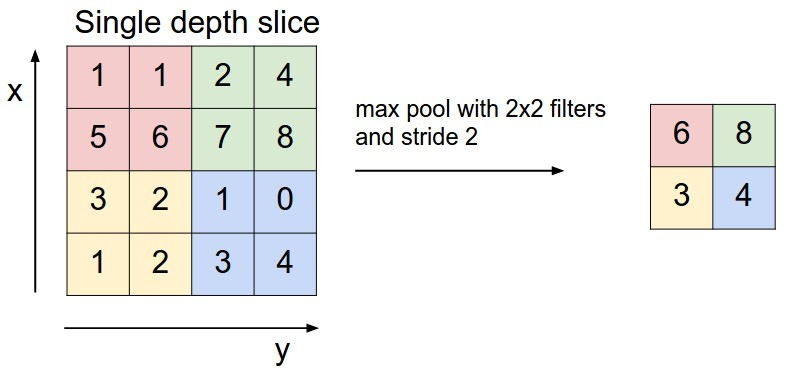
\includegraphics[width=0.6\columnwidth]{img/maxpool.jpeg}
%		\label{rr}
		\caption{The max-pooling layer.}
	\end{figure}

The pooling process introduces tolerance against shifts of the input patterns. Together with convolution layer it allows the CNN to detect if a particular event occurs, regardless its deformation or its position.

CNN is a feed-forward neural network \cite{726791} usually composed of three types of layers: convolutional layers, pooling layers and layers of neurons.
The convolutional layer performs the mathematical operation of convolution between a multi-dimensional input and a fixed-size kernel. Successively, a non-linearity is applied element-wise. 
%In the convolution process the kernel moves all along the input matrix and, for each position, every element of the kernel is multiplied with the corresponding one on the input matrix. All the values are finally summed.
The kernels are generally small compared to the input, allowing CNNs to process large inputs with few trainable parameters.
%From the input matrix, for each convolutional kernel, a new matrix is obtained, also called \textit{feature map}.
Successively, a pooling layer is usually applied, in order to reduce the feature map dimensions. One of the most used is the \textit{max-pooling} whose aim is to introduce robustness against translations of the input patterns.
%Different strategies are available for pooling, but we only consider max-pooling, which selects the maximum value in a sub-matrix of the input and discards the other values. Pooling introduces toughness against shifts of the input patterns. 
Finally, at the top of the network, a layer of neurons is applied. This layer does not differ from MLP, being composed by a set of activation and being fully connected with the previous layer. For clarity, the units contained in this layer will be referred as \textit{Hidden Nodes} (HN).

Denoting with $\mathbf{W}_{m} \in \mathbb{R}^{K_{1m}\times K_{2m}}$ the $m$-th kernel and with $\mathbf{b}_{m}  \in \mathbb{R}^{D_1\times D_2}$ the bias vector of a generic convolutional layer, the $m$-th feature map  $\mathbf{h}_{m} \in \mathbb{R}^{D_1\times D_2}$ is given by:
\begin{equation}\label{eq:backg:dnn:conv_op}
%h_{m,i}=\varphi	\left(W_{m,i} \ast \mathbf{u}_j[n] + b_{m,i} \right),
\mathbf{h}_{m}=\varphi	\left(\sum_{d=1}^{D_3} \mathbf{W}_{m} \ast \mathbf{u}_d + \mathbf{b}_{m} \right),
\end{equation}
where $\ast$ represent the convolution operation, and $\mathbf{u}_{d} \in \mathbb{R}^{D_1\times D_2} $ is a matrix of the three-dimensional input tensor $\mathbf{u} \in \mathbb{R}^{D_1\times D_2 \times D_3}$. The dimension of the $m$-th feature map $\mathbf{h}_{m}$ depends on the zero padding of the input tensor: here, padding is performed in order to preserve the dimension of the input, i.e., $\mathbf{h}_{m} \in \mathbb{R}^{D_1\times D_2}$. Please note that for the sake of simplicity, the time frame index $n$ has been omitted.  %The different feature maps obtained from each kernel of a convolutional layer are then summed to compose the input data for the following layer.
Commonly, \eqref{eq:backg:dnn:conv_op} is followed by a pooling layer in order to be more robust against patterns shifts in the processed data, e.g. a max-pooling operator that calculates the maximum over a $P_1 \times P_2 $ matrix is employed.

\end{enumerate}


A \textit{Deep Learning} definition: \textit{A  class  of  machine learning  techniques  that
exploit  many  layers  of  non-linear  information  processing  for supervised  or  unsupervised  feature  extraction  and  transformation, and for pattern analysis and classification.}
%...we need complex networks to deal with the \textit{feature representation learning} paradigm.
Artificial Neural Networks are often referred as deep when they have more than 1 or 2 hidden layers.
%		\item Important Issues
%		\begin{itemize}
%			\item Rule of Thumb: \textit{for a given performance rate on the testing data, the amount of training data and the number of free parameters are directly proportional}.
%			\item Do we have enough data for training and to achieve a satisfying generalization performance?
%			\item How to select the ``right'' model? 
%		\end{itemize}


\subsection{Stochastic gradient descent (SGD)}

Most deep learning training algorithms involve optimization of some sort.
The most widely used is the gradient based optimization, which belongs to the first order type.

\textit{Optimization} is the task of either minimizing some function $f(x)$ by altering $x$:
$f(x)$ is called \textit{objective function}, but in the case when it has to be minimized, it is also call the \textit{cost function}, \textit{loss function}, or \textit{error function}.
The aim of the optimization is reached doing small change $\epsilon$ in the input $x$, to obtain the corresponding change in the output $f(x)$:
\begin{equation}
f(x+\epsilon) \approx f(x)+\epsilon\,f'(x).
\end{equation}
This formulation is based on the calculation of the derivative $f'(x)$.
The \textit{gradient descent} is the technique based on the reduction of $f(x)$ by moving $x$ in small steps with the opposite sign of the derivative.
The aim is to find the minimum of the cost function: when $f'(x)=0$, the derivative provides no information about which direction to move, therefore this point is defined as stationary points.
A local minimum is a point where $f(x)$ is lower than at all neighbouring and it is no longer possible to decrease $f(x)$ by making infinitesimal steps.
The absolute lowest value of $f(x)$ is a \textit{global minimum}.

For the concept of minimization to make sense, there must still be only one (scalar) output.
For functions that have multiple inputs $f: \R^n \rightarrow \R$, the concept of \textit{partial derivatives} is introduced.
The gradient $\nabla_{\mathbf{x}}f(\mathbf{x})$ is the vector containing all the partial derivatives.

The method of \textit{steepest descent} or \textit{gradient descent} states that decrease $f$ by moving in the direction of the negative gradient.
\begin{equation}
\textbf{x'} = \textbf{x} - \epsilon\,\nabla_{\mathbf{x}}f(\mathbf{x}),
\end{equation}
where $\epsilon$ is the \textit{learning rate}, a positive scalar determining the size of the step.

Large training sets are necessary for good generalization, but large training sets are also more computationally expensive.
The cost function decomposes as a sum over training example of per-example loss function:
i.e., the negative conditional log-likelihood of the training data is defined as:
\begin{equation}
J(\mathbf{\theta}) = \mathbb{E}(L(\textbf{x}, y, \mathbf{\theta})) = \frac{1}{m} \sum\limits_{i=1}^{m} L(\textbf{x}^{(i)}, y^{(i)}, \mathbf{\theta}),
\end{equation}
where $L$ is the per-example loss $L(\textbf{x}, y, \mathbf{\theta}) = - \log p(y|\textbf{x};\mathbf{\theta})$.
The gradient descent requires computing:
\begin{equation}
\nabla_{\theta} J(\mathbf{\theta}) = \frac{1}{m} \sum\limits_{i=1}^{m} \nabla_{\theta} L(\textbf{x}^{(i)}, y^{(i)}, \mathbf{\theta}).
\end{equation}
The computational cost of this operation is proportional to the number of example $m$, therefore as the training set size grows the time to take a single gradient step becomes prohibitively long.

\textit{Stochastic gradient descent} (SGD) is an extension of the gradient descent algorithm: the insight is that the gradient is an expectation estimated using a small set of samples.
On each step of the algorithm, a sample of example $\mathbb{B} = \{ \textbf{x}^{(1)}, \ldots, \textbf{x}^{(m')}\}$, called \textit{minibatch}, is drawn uniformly from the training set.
The minibatch size $m'$ is typically chosen to be a relatively small number of examples.
The estimate of the gradient is:
$\textbf{g} = \frac{1}{m'} \nabla_{\theta} \sum\limits_{i=1}^{m'} L(\textbf{x}^{(i)}, y^{(i)}, \mathbf{\theta})$
using examples from the minibatch $\mathbb{B}$.
The SGD algorithm then follows the estimated gradient downhill:
\begin{equation}
\theta \leftarrow \theta - \epsilon\,\textbf{g}
\end{equation}
where $\epsilon$ is the learning rate.

%\textbf{ndRob} to be inserted: tipo di loss function MSE, come si calcola su uscita 

%\textbf{ndRob} to complete, learning for FF e CNN (in slides)




\subsection{Autoencoder}

%\textbf{ndRob} to complete, 1-2 pages with figures
%
%\begin{itemize}
%\item definition
%\item notazione matriciale
%\item denoising Auto Encoder (dAE)
%\end{itemize}



An Autoencoder is a kind of neural network typically consisting of only one hidden layer, trained to set the target values to be equal to the inputs.
\begin{equation} %\label{eq:layer2}
  \tilde{x} = f(W_{2}h(x) +b_{2})
\end{equation}
 
%\begin{figure}
%\centering
%\includegraphics[width=0.65\textwidth]{img/basic_AE}
%%\label{ee}
%\caption{rr}
%\end{figure}


Given an input set of examples $\mathcal{X}$, autoencoder training consists
in finding parameters $\theta=\{W_{1},W_{2},b_{1},b_{2}\}$ that
minimize the Reconstruction Error:
\begin{equation}\label{eq:obAE}
  \mathcal{J}(\theta)=\sum_{x\in{\mathcal{X}}}\left\| x - \tilde{x}\right\|^{2}
\end{equation}

Defining $M$ the number of hidden units, and $N$ the number of input units, output units, features size:

\begin{figure}
\centering
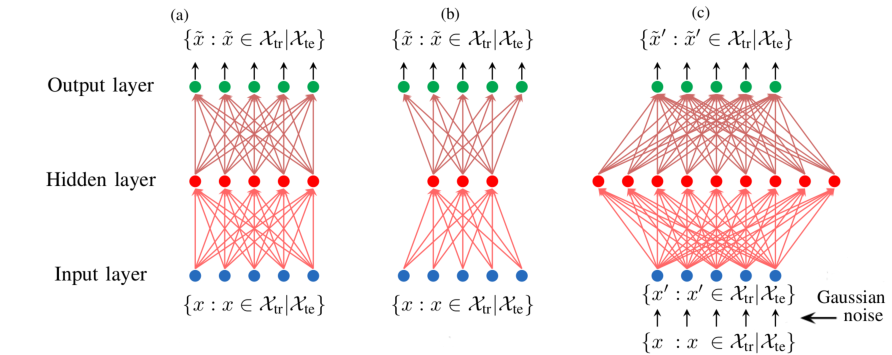
\includegraphics[width=\columnwidth]{img/autoencoders}
\caption{The different types of Autoencoders.}
\label{fig:backg:dnn:AE}
\end{figure}

\begin{itemize}
\item (a):  $M=N \rightarrow$ Basic Autoencoder (AE);
\item (b):  $M<N \rightarrow$ Compression Autoencoder (CAE);
\item (c):  $M>N$ and Gaussian Noise $\rightarrow$ Denoising Autoencoder (DAE);
\end{itemize}


%This section introduces the concepts of autoencoders and describes the basic autoencoder, compression autoencoder, de-noising autoencoder, and non-linear predictive autoencoder.


\subsubsection{Basic Autoencoder}
A basic AE -- a kind of neural network typically consisting of only one hidden layer --, sets the target values to be equal to the input. It is used to find common data representation from the input \cite{Goodfellow2009-MII,Bengio2007-GLT}. Formally, in response to an input example $x\in \mathbf{R}^{n}$, the hidden representation
$h(x) \in \mathbf{R}^{m}$ is 
\begin{equation} %\label{eq:layer1}
  h(x) = f(W_{1}x +b_{1}), 
\end{equation}
where $f(z)$ is a non-linear activation function, typically a logistic
sigmoid function $f(z) = 1/(1+\exp(-z)) $ applied component-wisely,
$W_{1} \in \mathbf{R}^{m \times n}$ is a weight matrix, and $b_{1} \in
\mathbf{R}^{m}$ is a bias vector.

The network output maps the hidden representation $h$ back to a
reconstruction $\tilde{x} \in \mathbf{R}^{n}$:
\begin{equation} %\label{eq:layer2}
  \tilde{x} = f(W_{2}h(x) +b_{2}), 
\end{equation}
where $W_{2} \in \mathbf{R}^{n \times m}$ is a weight matrix, and $b_{2} \in
\mathbf{R}^{n}$ is a bias vector.

Given an input set of examples $\mathcal{X}$, AE training consists
in finding parameters $\theta=\{W_{1},W_{2},b_{1},b_{2}\}$ that
minimise the reconstruction error, which corresponds to minimising
the following objective function:
\begin{equation} %\label{eq:obAE}
  \mathcal{J}(\theta)=\sum_{x\in{\mathcal{X}}}\left\| x -
    \tilde{x}\right\|^{2}.
\end{equation}
The minimisation is usually realised by stochastic gradient descent as
in the training of neural networks. The structure of the AE is given in \figref{fig:backg:dnn:AE}a.   

\subsubsection{Compression Autoencoder}
In the case of having the number of hidden units $m$ smaller than the number of input units $n$, the network is forced to
learn a compressed representation of the input. For example, if some of the input features are correlated, then this compression autoencoder (CAE) is able to learn those correlations and reconstruct the input data from a compressed representation. The structure of the CAE is given in \figref{fig:backg:dnn:AE}b.

\subsubsection{De-noising Autoencoder}\label{sssec:backg:dnn:dAE}
The de-noising AE (DAE) \cite{Vincent10-SDA} forces the hidden layer to retrieve more robust features and prevent it from simply learning the identity. In such a configuration the AE is trained to reconstruct the original input from a corrupted version of it. Formally, the initial input $x$ is corrupted by means of additive isotropic Gaussian noise in order to obtain: $x'|x \sim N(x,\sigma^2I)$. The corrupted input $x'$ is then mapped, as with the AE, to a hidden representation
\begin{equation} %\label{eq:layer11}
  h(x') = f(W'_{1}x' +b'_{1}), 
\end{equation}
from which the original signal is reconstructed as follows:
\begin{equation} %\label{eq:layer12}
  \tilde{x}' = f(W'_{2}x +b'_{2}). 
\end{equation}
The parameters $\theta'=\{W'_{1},W'_{2},b'_{1},b'_{2}\}$ are trained to minimise the average reconstruction error over the training set, to have $\tilde{x}'$ reach as close as possible to the uncorrupted input $x$, which corresponds to minimising the objective function in Equation \ref{eq:obAE}.
%%%%%%%%%%%%%%%%%%%%%%%%%
The structure of the de-noising autoencoder is shown in \figref{fig:backg:dnn:AE}c.





%\textbf{ndRob} descrizione teorica dAE 1D, from paper Neural NILM, 









\graphicspath{{3_datasets_and_evaluation/}}
\chapter{Datasets and Evaluation}\label{ch:datasets}
Every problem to be solved with machine learning and data mining techniques
requires the availability of data for algorithm parametrization: the ability to
access public dataset, representative of a real scenario, allows to test the approaches, in order to evaluate the effective benefit in real applications, and
to compare the performance of existing approaches on a common comparison
basis. A reliable
evaluation procedure for a classification or recognition system will involve a
standard dataset of example input data along with the intended target output, and
well-defined metrics to compare the systems’ outputs with this ground truth. 

%TODO Define typical characteristics of dataset acquisition

\section{Datasets for Sound Event Detection}
In order to evaluate the proposed method in polyphonic real-life conditions, we used the TUT Sound Events 2016 \& 2017 datasets, which were included in the corresponding editions of the DCASE Challenge. For the monophonic-SED case study, we used the TUT Rare Sound Events 2017 which represents the task 2 of the DCASE 2017 Challenge.

\subsubsection{TUT Sound Events 2016}
The TUT Sound events 2016 (TUT-SED 2016)\footnote{\url{http://www.cs.tut.fi/sgn/arg/dcase2016/}} dataset consists of recordings from two acoustic scenes, respectively ``Home'' (indoor) and ``Residential area'' (outdoor) which we considered as two separate subsets. These acoustic scenes were selected from the challenge organizers to represent common environments of interest in applications for safety and surveillance (outside home) and human activity monitoring or home surveillance \cite{mesaros2016tut}.
%The dataset was collected in Finland by Tampere University of Technology from different locations by means of a binaural recording system. For each location, a 3-5 minute long binaural
%audio recording is provided for a total of around 54 and 59 minutes of audio respectively for ``Home'' and ``Residential area'' scenario.
A total amount of around 54 and 59 minutes of audio are provided respectively for ``Home'' and ``Residential area'' scenarios.
Sound events present in each recording were manually annotated without any further cross-verification, due to the high level of subjectivity inherent to the problem. 
For the ``Home'' scenario a total of 11 classes were defined, % (including Object impact, People walking, Washing dishes),
while for the ``Residential Area'' scenario 7 classes were annotated. % (including Bird singing, Car passing by, People speaking).

Each scenario of the TUT-SED 2016 has been divided into two subsets: development dataset and evaluation dataset. The split was done based on the number of examples available for each sound event class. In addition, for the development dataset a cross-validation setup is provided in order to easily compare the results of different approaches on this dataset. The setup consists of 4 folds, so that each recording is used exactly once as test data. In detail, ``Residential area'' sound events data consists of 5 recordings in the evaluation set and 12 recordings in the development set while ``Home'' sound events data consists of 5
recordings in the evaluation set and 10 recordings in turn divided into 4 folds as training and validation subsets.


\subsubsection{TUT Sound Events 2017}
The TUT Sound Events 2017 (TUT-SED 2017)\footnote{\label{note_dcase17}\url{http://www.cs.tut.fi/sgn/arg/dcase2017/}} dataset consists of recordings of street acoustic scenes with various levels of traffic and other activities, for a total of 121 minutes of audio. The scene was selected as representing an environment of interest for detection of sound events related to human activities and hazard situations. It is a subset of the TUT Acoustic scenes 2016 dataset \cite{mesaros2016tut}, from which also TUT-SED 2016 dataset was taken. Thus, the recording setup, the annotation procedure, the dataset splitting, and the cross-validation setup is the same described above. The 6 target sound event classes were selected to represent common sounds related to human presence and traffic, and they include brakes squeaking, car, children, large vehicle, people speaking, people walking. The evaluation set of the TUT-SED 2017 consists of 29 minutes of audio, whereas the development set is composed of 92 minutes of audio which are employed in the cross-validation procedure.

\subsubsection{TUT Rare Sound Events 2017} 
The TUT Rare Sound Events 2017 (TUT-Rare 2017)\textsuperscript{\ref{note_dcase17}} \cite{DCASE2017challenge} consists of isolated sounds of three different target event classes (respectively, baby crying, glass breaking and gunshot) and 30-second long recordings of everyday acoustic scenes to serve as background, such as park, home, street, cafe, train, etc. \cite{mesaros2016tut}. In this case we consider a \textit{monophonic}-SED, since the sound events are artificially mixed with the background sequences without overlap. In addition, the event potentially present in each test file is known a-priori thus it is possible to train different models, each one specialized for a sound event. In the development set, we used a number of sequences equal to 750, 750 and 1250 for training respectively of the baby cry, glass-break and gunshot models, while we used 100 sequences as validation set and 500 sequences as test set for all of them. In the evaluation set, the training and test sequences of the development set are combined into a single training set, while the validation set is the same used in the Development dataset. The system is evaluated against an ``unseen'' set of 1500 samples (500 for each target class) with a sound event presence probability for each class equal to 0.5.

\subsection{Snore Sound Detection in Real Life Audio}
\label{ssec:dataset}
The snore detection algorithm has been evaluated on the A3-Snore dataset. A brief description of the acquisition setup and dataset splitting is provided in the following.

\subsubsection{Acquisition setup:}
In order to capture the overnight audio recordings a ZOOM-H1 Handy Recorder has been used. It is equipped with two unidirectional microphones set at a 90 degree angle relative to one another. The signals are stored in WAV files with a sampling rate of 44.1\ kHz and bit depth equal to 16.
The input gain is automatically set by the recorder to prevent overload and distortion, while the high-pass filter was enabled in order to eliminate pops, wind noise, blowing, and other kinds of low frequency rumble.


\subsubsection{Acquisition environment:}
The acquisition environment consist of a simple bedroom, with two access points (door and window). The recorder is placed near the patient, at same height of the bed and in line with the subject's mouth. During the recordings, the patient is the only one that can occupy the bedroom, in order to avoid contaminations on recorded audio signals. The room dimensions are reported in \figref{fig:room}.
Background sounds include traffic noise, breathing and speech signals, house and animal noises. We acquired some samples measurements of the event-to-background (EBR) ratios considering background noise, snoring events and noise events such as ``car passing by'' or ``dog barfing''. The EBR resulted equal to 6.5 dB and 1.1 dB respectively for noise to background EBR and snore to background EBR. 


\begin{figure}[t]
	\centering
	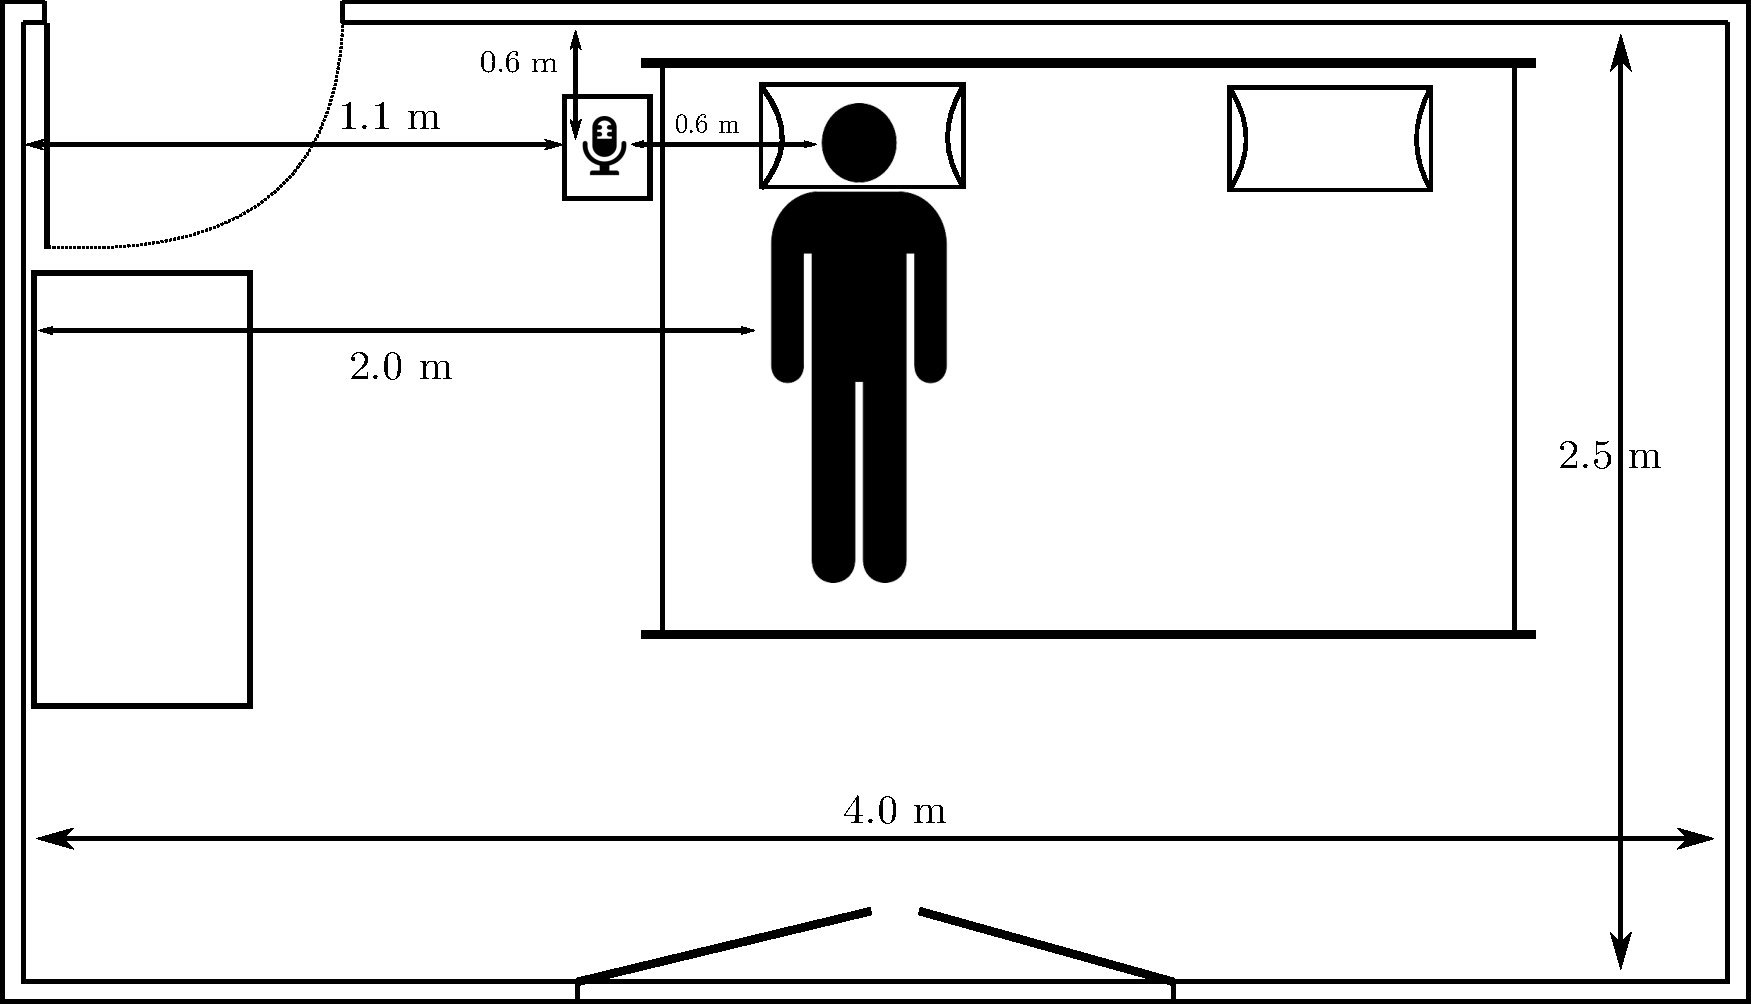
\includegraphics[width=0.8\columnwidth]{img/room.pdf}
	\caption{Plant of the recording room.} 
	\label{fig:room}
\end{figure}


\subsubsection{Dataset splitting:}
The original recordings have been manually labelled, annotating the snore events onset and offset with a resolution of 1 second. The audio sequences have been divided into chunks of 10 minutes, and only those with the highest number of snore events have been used in the experiments. 
The dataset is organized into subjects, which can be respectively used as \emph{training} or \emph{validation} sets in a two fold cross validation strategy (i.e., Leave One Subject Out procedure). The number of events per class in the database is strongly unbalanced as reported in \tableref{a3snore}. Thus, the snore detection task is challenging, due to the high number of noises on the A3-SNORE dataset. 

\begin{table}[ht]
	\centering
	\caption[A3-SNORE dataset]{Difference of recording times for each class, divided by snorers.}
	\begin{tabular}{cccccc}
		\hline
		\multicolumn{6}{c}{\textbf{A3-SNORE dataset}} \\
		\hline
		\# & Gender & Age & Snoring (SN) & Total Duration (Tot) & Ratio (SN/Tot) \\
		\hline
		Snorer 1 & M & 48 & 33m-27s & 3h-12m-0s & 14.5\% \\
		Snorer 2 & M & 55 & 21m-21s & 3h-50m-0s & 11.1\% \\
		\hline
		\multicolumn{3}{l}{Total} &	54m-48s	& 7h-02m-0s	& 12.8\%\\
		\hline    
	\end{tabular}	
	\label{a3snore} 
\end{table}

\subsection{Acoustic Novelty Detection}

\label{sec:databases}
This section describes the three databases evaluated in our experiments: A3Novelty, PASCAL CHiME, and PROMETHEUS.

\subsubsection{A3NOVELTY}

%FABIO Description of A3Corpus taken from ESWA paper. Io l'ho parafrasata in modo "light"...vedete voi se bisogna modificarla di più.

%TODO: add description of the database.

%TODO: add final table including stats on the datasets (number of abnormal sounds, duration etc...


The A3Novelty corpus\footnote{\label{note:a3}\url{http://www.a3lab.dii.univpm.it/research/a3novelty}} includes around 56 hours of recording acquired in a laboratory of the Università Politecnica delle Marche. 
These recordings were performed during different day and night hours, so very different acoustic conditions are available.
A variety of \emph{novel} events were randomly played back by a speaker (e.g., scream, fall, alarm or breakage of objects) during the recordings.

Eight microphones were used in the recording room for the acquisitions: four Behringer B-5 microphones with cardioid pattern and an
array of four AKG C400 BL microphones spaced by 4\,cm, then A MOTU 8pre sound card and the NU-Tech software were utilised 
to record the microphone signals. The sampling rate was equal to 48\,kHz.


The abnormal event sounds (cf.  Table \ref{tab:events}) can be grouped into four categories and they are freely available to download from \url{http://www.freesound.org}:
\begin{itemize}
	\item \textit{Sirens}, three different types of sirens or alarm sounds.
	\item \textit{Falls}, two occurrences of a person or an object falling to the ground.
	\item \textit{Breakage of objects}, noise produced by the breakage of an object after the impact with the ground.
	\item \textit{Screams}, four different human screams, both produced by a single person or by a group of people.
\end{itemize}


The A3Novelty corpus is composed of two types of recordings:
\emph{background}, which contains only background sounds such as human speech, technical tools noise and environmental sounds and \emph{background with novelty}, which contains in addition to the background the artificially generated novelty events.

In the original A3Novelty database the recordings are segmented in sequences of 30 seconds. In order to limit the size of training data, we randomly selected 300 sequences from the \emph{background} partition to compose of training material (150 minutes), and 180 sequences from the \emph{background with novelty} partition to compose the testing set (90 minutes). The test set contains 13 novelty occurrences.

For reproducibility, the list of randomly selected recordings, as well as the train and test set are made available % \footnotemark[\ref{note:a3}]. %ndFAB\footnotemark [3].


%\begin{table}[t]
%\centering
%\begin{tabular}{lccc}
%\hline
%\textbf{Rec Type} & \textbf{Day/Night} & \textbf{Length (hh:mm)} & \textbf{Novelty events}\\
%\hline
%\multirow{2}{*}{Background} & Day & 12:00 & -\\
%& Night & 24:00 & -\\
%\hline
%Background & Day & 9:00 & 16\\
%with novelty & Night & 12:00 & 30\\
%\hline
%\end{tabular}
%\caption{Recordings details.}
%\label{tab:recs_detail}
%\end{table}


\subsubsection{PASCAL CHiME}
\label{subsec:pascal}

The original dataset is composed of around 7 hours of recordings of a home environment, taken from the PASCAL CHiME speech separation and recognition challenge \cite{barker2013pascal}. 
It consists of a typical in-home scenario (a living room), recorded during different days and times,
while the inhabitants (two adults and two children) perform common actions, such as talking, watching television, playing, or eating. The dataset was recorded in stereo (with a binaural microphone) and a sample-rate of 16\,kHz. In the original PASCAL CHiME database the recordings are segmented in sequences of 5 minutes duration. In order to limit the size of training data, we randomly selected sequences to compose 100 minutes of background for the training set, and around 70 minutes for the testing set. For reproducibility, the list of randomly selected recordings, as well as the train and test set are made available\footnote{\url{http://a3lab.dii.univpm.it/webdav/audio/Novelty_Detection_Dataset.tar.gz}}. 
%The test set was generated adding different kinds of sounds\footnote{taken from www.freesound.org}, such as screams, alarms, falls and fractures (cf.\ Table \ref{tab:events}). 
%The test set did not include any overlapping events, the events were  and they were added at random position thus the distance between one event and another is not fixed. %ndFAB\footnotemark [1].
% %VES
The test set was generated adding different typologies of sounds\footnote{taken from www.freesound.org}, such as screams, alarms, falls and fractures (cf.\ Table \ref{tab:events}), after their normalization to the volume of the background recordings. % %
The events in the test set were added at random position (avoiding overlapping), thus the distance between one event and another is not fixed. %ndFAB\footnotemark [1].




\subsubsection{PROMETHEUS}
\begin{table}[t]
	\centering
	\tabcolsep=0.10cm
	\renewcommand{\arraystretch}{1.0}
	\caption[Acoustic novel events]{Acoustic novel events in the test set. Shown are the number of different events per database, the average duration, and the total duration in seconds per event type. The last column indicates the total number of events and total duration across the databases. The last line indicates the total duration in seconds of the test set including normal and novel events per database.}
	
	\begin{tabular}{ l || c c || c c || c c | c c | c c | c c || c c }
		\textbf{Events} & \multicolumn{2}{|c||}{A3Novelty} & \multicolumn{2}{|c||}{PASCAL CHiME} & \multicolumn{8}{|c||}{PROMETHEUS} & \multicolumn{2}{|c}{Total}\\
		\textbf{} & \multicolumn{2}{|c||}{} & \multicolumn{2}{|c||}{} & \multicolumn{2}{|c|}{ATM} & \multicolumn{2}{|c|}{Corridor} & \multicolumn{2}{|c|}{Outdoor} & \multicolumn{2}{|c||}{Smart-room} & \multicolumn{2}{|c}{}\\
		\textbf{} & \# & time(avg.) & \# & time(avg.) & \# & time(avg.) & \# & time(avg.) & \# & time(avg.) & \# & time(avg.) & \# & time\\
		\hline
		Alarm			& - & -		& 76 & 435.8 (6.0) 	 				& - & -			& 6 & 84.0 (14.0)	& - & -				& 3 & 9.0 (3.0)		& 85 & 528.8\\
		Anger			& - & - 				& - & - 				& - & -			& - & -				& 6 & 293.0 (48.8)		& - & - 			& 6 & 293.0\\  
		Fall 			& 3 & 4.2 (2.1)		& 48 & 89.5 (1.8) 	& - & -	 		& 3 & 3.0 (1.0)		& - & -				& 2 & 2.0 (1.0) 		& 55 & 98.7\\
		Fracture		& 1 & 2.2 			& 32 & 70.4 (2.2) 	& - & - 			& - & -				& - & -				& - & - 				& 33 & 72.6\\
		Pain			& - & -			 	& - & - 			& - & -	 		& 2 & 8.0 (4.0)		& - & -				& 5 & 67.0 (13.4) 		& 7 & 75.0\\
		Scream			& 6 & 10.4(1.7)		& 111 & 214.6 (1.9) 	& 5 & 30.0 (6.0)	& 25 & 228.0 (9.1)	& 4 & 48.0 (12.0)		& 10 & 234.0 (23.4) & 159 & 762.2\\
		Siren			& 3 & 20.4 (6.8)		& - & - 				& - & - 			& - & -				& - & -				& - & -				& 3 & 18.1\\
		\hline
		Total			& 13 & 38.1 (2.9) & 267 & 810.3 (3.1) 	& 5 & 30.0 (5.0) 		& 36 & 323.0 (9.0) 	& 10 & 341.0 (34.1) 	& 20 & 312.0 (15.6) & 348 & 1848.4\\
		\hline\hline
		Test time & - & 5400.0 				& - & 4188.0 	& - & 750.0			& - & 960.0	& - & 1620.0				& - & 1020.0		& - & 13938.0\\
		
	\end{tabular}
	\label{tab:events}
\end{table}

The PROMETHEUS database \cite{ntalampiras:probabilistic} contains recordings of various scenarios designed to serve a wide range of real-world applications. The database includes: 1) a \textit{smart-room} indoor home environment including phases where a user is interacting with an automated speech-driven home assistant, 2) an outdoor public space consisting of \textit{a}) interaction of people with an \textit{ATM}, \textit{b}) an \textit{outdoor} security scenario in which people are waiting in front of a counter, and 3) an  indoor office \textit{corridor} scenario for security monitoring in standard indoor space. 
%The first one is intended to be representative of particular activities which take place inside an intelligent environment, including phases where the user is interacting with an automated speech-driven home assistant. As for the second setting, two scenarios with different scopes were captured: 1) ATM scenario, which included interactions of people with an ATM, and 2) security scenario, in which people in a queue are waiting for service in front of a counter and can be utilized as a general-purpose scenario with many applications (e.g., bank, airport, etc.). The third setting was used for security scenarios in a standard indoors space. 
These scenarios substantially differ in terms of acoustic environment. The indoor scenarios were recorded under quiet acoustic conditions, whereas the outdoor recordings were conducted in an open-air public area and contain non-stationary background noise.   
The smart-home scenario contains recordings of five professional actors performing five single-person and 14 multiple-person action scripts. The main activities include human-machine interaction with a virtual home agent, a number of alternating normal and abnormal activities specifically designed to monitor and interpret human behaviour. The single-person and multiple-person actions include abnormal events, such as: falls, alarm followed by panic, atypical vocalic reactions (pain, fear, anger), or fractures. Examples are: walking to the couch, sitting or interacting with the smart environment to turn the TV on, open the windows, or decrease the temperature. The scenarios were recorded three to five times, by changing the actors and their roles in the action scripts.
Table \ref{tab:events} provides details on the number of abnormal events per scenario, including average time duration.


\section{The DIRHA Dataset}
\label{sec:dataset}

\begin{figure}[h]
	\centering
	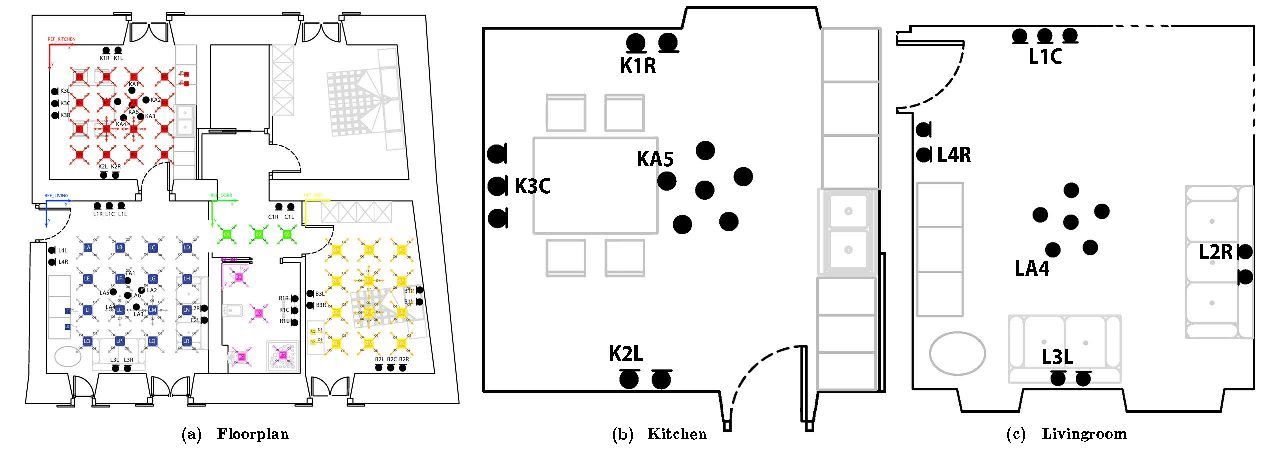
\includegraphics[width=\textwidth]{img/plan}
	\caption{The map of the apartment used for the DIRHA project (a). Figures (b) and (c) show the considered rooms, with the disposition of their relative microphones. }
	\label{fig:DIRHA_map}
\end{figure}

The analysis of the DNN-SLOC performance has been conducted on the DIRHA dataset \cite{cristoforetti2014dirha}, characterized by diverse scenes, rooms, microphones and noise conditions\footnote{\url{http://dirha.fbk.eu/simcorpora}}. In details, the apartment where the dataset has been recorded consists in five rooms and a total of 40 microphones. These are arranged in linear and circular arrays, with the first ones placed on the walls of all rooms, and the circular ones are placed on the ceiling of the living room and of the kitchen (\figref{fig:DIRHA_map}).

The dataset is composed of two subsets, named \emph{Simulated} and \emph{Real}. For each of them several \textit{scenes} have been recorded, composed of typical situations observable in a domestic context. As reported in \tableref{tab:dataset}, the two subsets differ in terms of scenes and total length: in the Simulated set the scenes length is fixed to 60 seconds, while it varies in the Real set. In addition, the latter has been recorded with persons moving in the rooms and speaking towards different directions throughout the scenes, whilst the Simulated has been obtained by convolving a fixed set of measured Room Impulse Responses (RIRs) with recorded signals.
The Simulated subset is also characterized by a lower SNR compared to the Real one and overlapping speech does not occur.

Our study focuses on two rooms of the dataset, i.e.,  the Kitchen and the Living Room, due to three main aspects. First of all, these rooms consist in the area of a home-environment where most of the events take place. In addition, being the widest rooms of the apartment, the localization task is more challenging. \textcolor{red}{The room dimensions are respectively $4.79$\,m~$\times$~$3.80$\,m for the Kitchen and $4.79$\,m~$\times$~$4.85$\,m for the Living Room.}
Finally, the number of microphones are higher compared to the other rooms, and they comprise both wall and ceiling arrays.

\begin{table}[t]
	%\renewcommand{\arraystretch}{1.2}
	\centering
	%	\small
	\caption{Main differences between the Real and Simulated subsets.}
	\resizebox{.75\columnwidth}{!}{%
		\begin{tabular}{c|c|c}\hline
			& \textbf{Real} & \textbf{Simulated} \\ \hline
			\textbf{Nr.\ of Scenes}  & 22 & 80 \\ \hline
			
			\textbf{Total Duration} &  21.5 min. & 80 min.  \\  \hline
			\multirow{2}{*}{\textbf{Speech Percentage}}	&  12.9\%  & 23.6\%  \\
			& 	2.8  min.	& 18.9 min. \\ \hline
			\textbf{Source} & human (moving) & loudspeaker (static) \\ \hline
			\textbf{Background} & quiet & various \\ \hline
			\textbf{Noise Source Rate} & low & high \\ \hline
			\textbf{Overlapping Events} & no & yes \\ \hline  
		\end{tabular} 
	}
	\label{tab:dataset}
\end{table}

\section{Datasets for Sound Event Classification}

\subsection{Acoustic Road Roughness Classification}
The dataset built for this work is done with a multi-channel microphone arrangement, with the prospect of conducting different assessments at once or to exploit microphone diversity to improve the classification. More specifically, two microphones have been placed close to the rear wheels, one in front of the front left wheel, one inside the engine compartment and two inside the cockpit, close to the driver head and close to the right passenger head. The rear wheel microphones have been placed off-axis, in order to avoid dirt from the wheel and protected by the wheelhouse to reduce the effect of wind. Figure \ref{fig:car-mic} shows the positioning of all microphones. External microphones are \textit{PCB Piezotronics} model 130A24. These are IP55 microphones and they have been protected with a melamine resin foam for sound absorption to reduce the effect of wind. The internal microphones are \textit{PCB Piezotronics} model 378C20. The front-right wheel has been excluded from recordings after first informal evaluations because it picked a large amount of engine noise with respect to the other microphones. The rear-right microphone, vice versa, was found to be the best choice because the noise from the engine was the lowest and it has been used for this first evaluation. The engine compartment microphone has been used to record the engine conditions for future use. In \figref{fig:car-rr-and-fl} are shown the images of the microphones installation. 

\begin{figure}[ht]
	\centering
	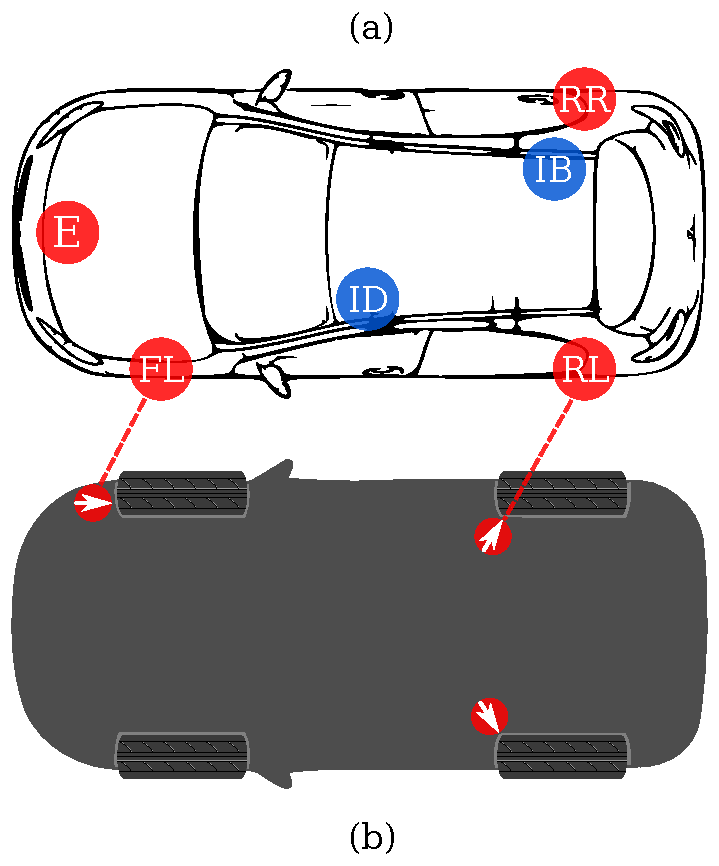
\includegraphics[width=0.5\textwidth]{img/car-mic}
	\caption[Position of the microphones in the car used to record the dataset]{Positioning of the microphones in the car used to record the dataset, top view (a) and bottom view (b). The microphones are placed in the engine compartment (E), close to the front-left, rear-left and rear-right tyres (FL, RL, RR), and inside the car close to the driver or in the back seat (ID, IB). The last two microphones are \textit{PCB Piezotronics} model 378C20 type microphones, while all the others are IP55 \textit{PCB Piezotronics} model 130A24 microphones. The microphones are omnidirectional, however the arrows in (b) show how the capsule was positioned to minimize wind effect. The rear microphones are protected in the wheelhouse.}
	\label{fig:car-mic}
\end{figure}

\begin{figure}[t]
	\centering
	\begin{subfigure}[b]{0.48\textwidth}
		\includegraphics[width=\textwidth]{img/Rear-Right.jpg}
		\subcaption{Rear right tyre microphone.}
	\end{subfigure}
	\hfil
	\begin{subfigure}[b]{0.48\textwidth}
		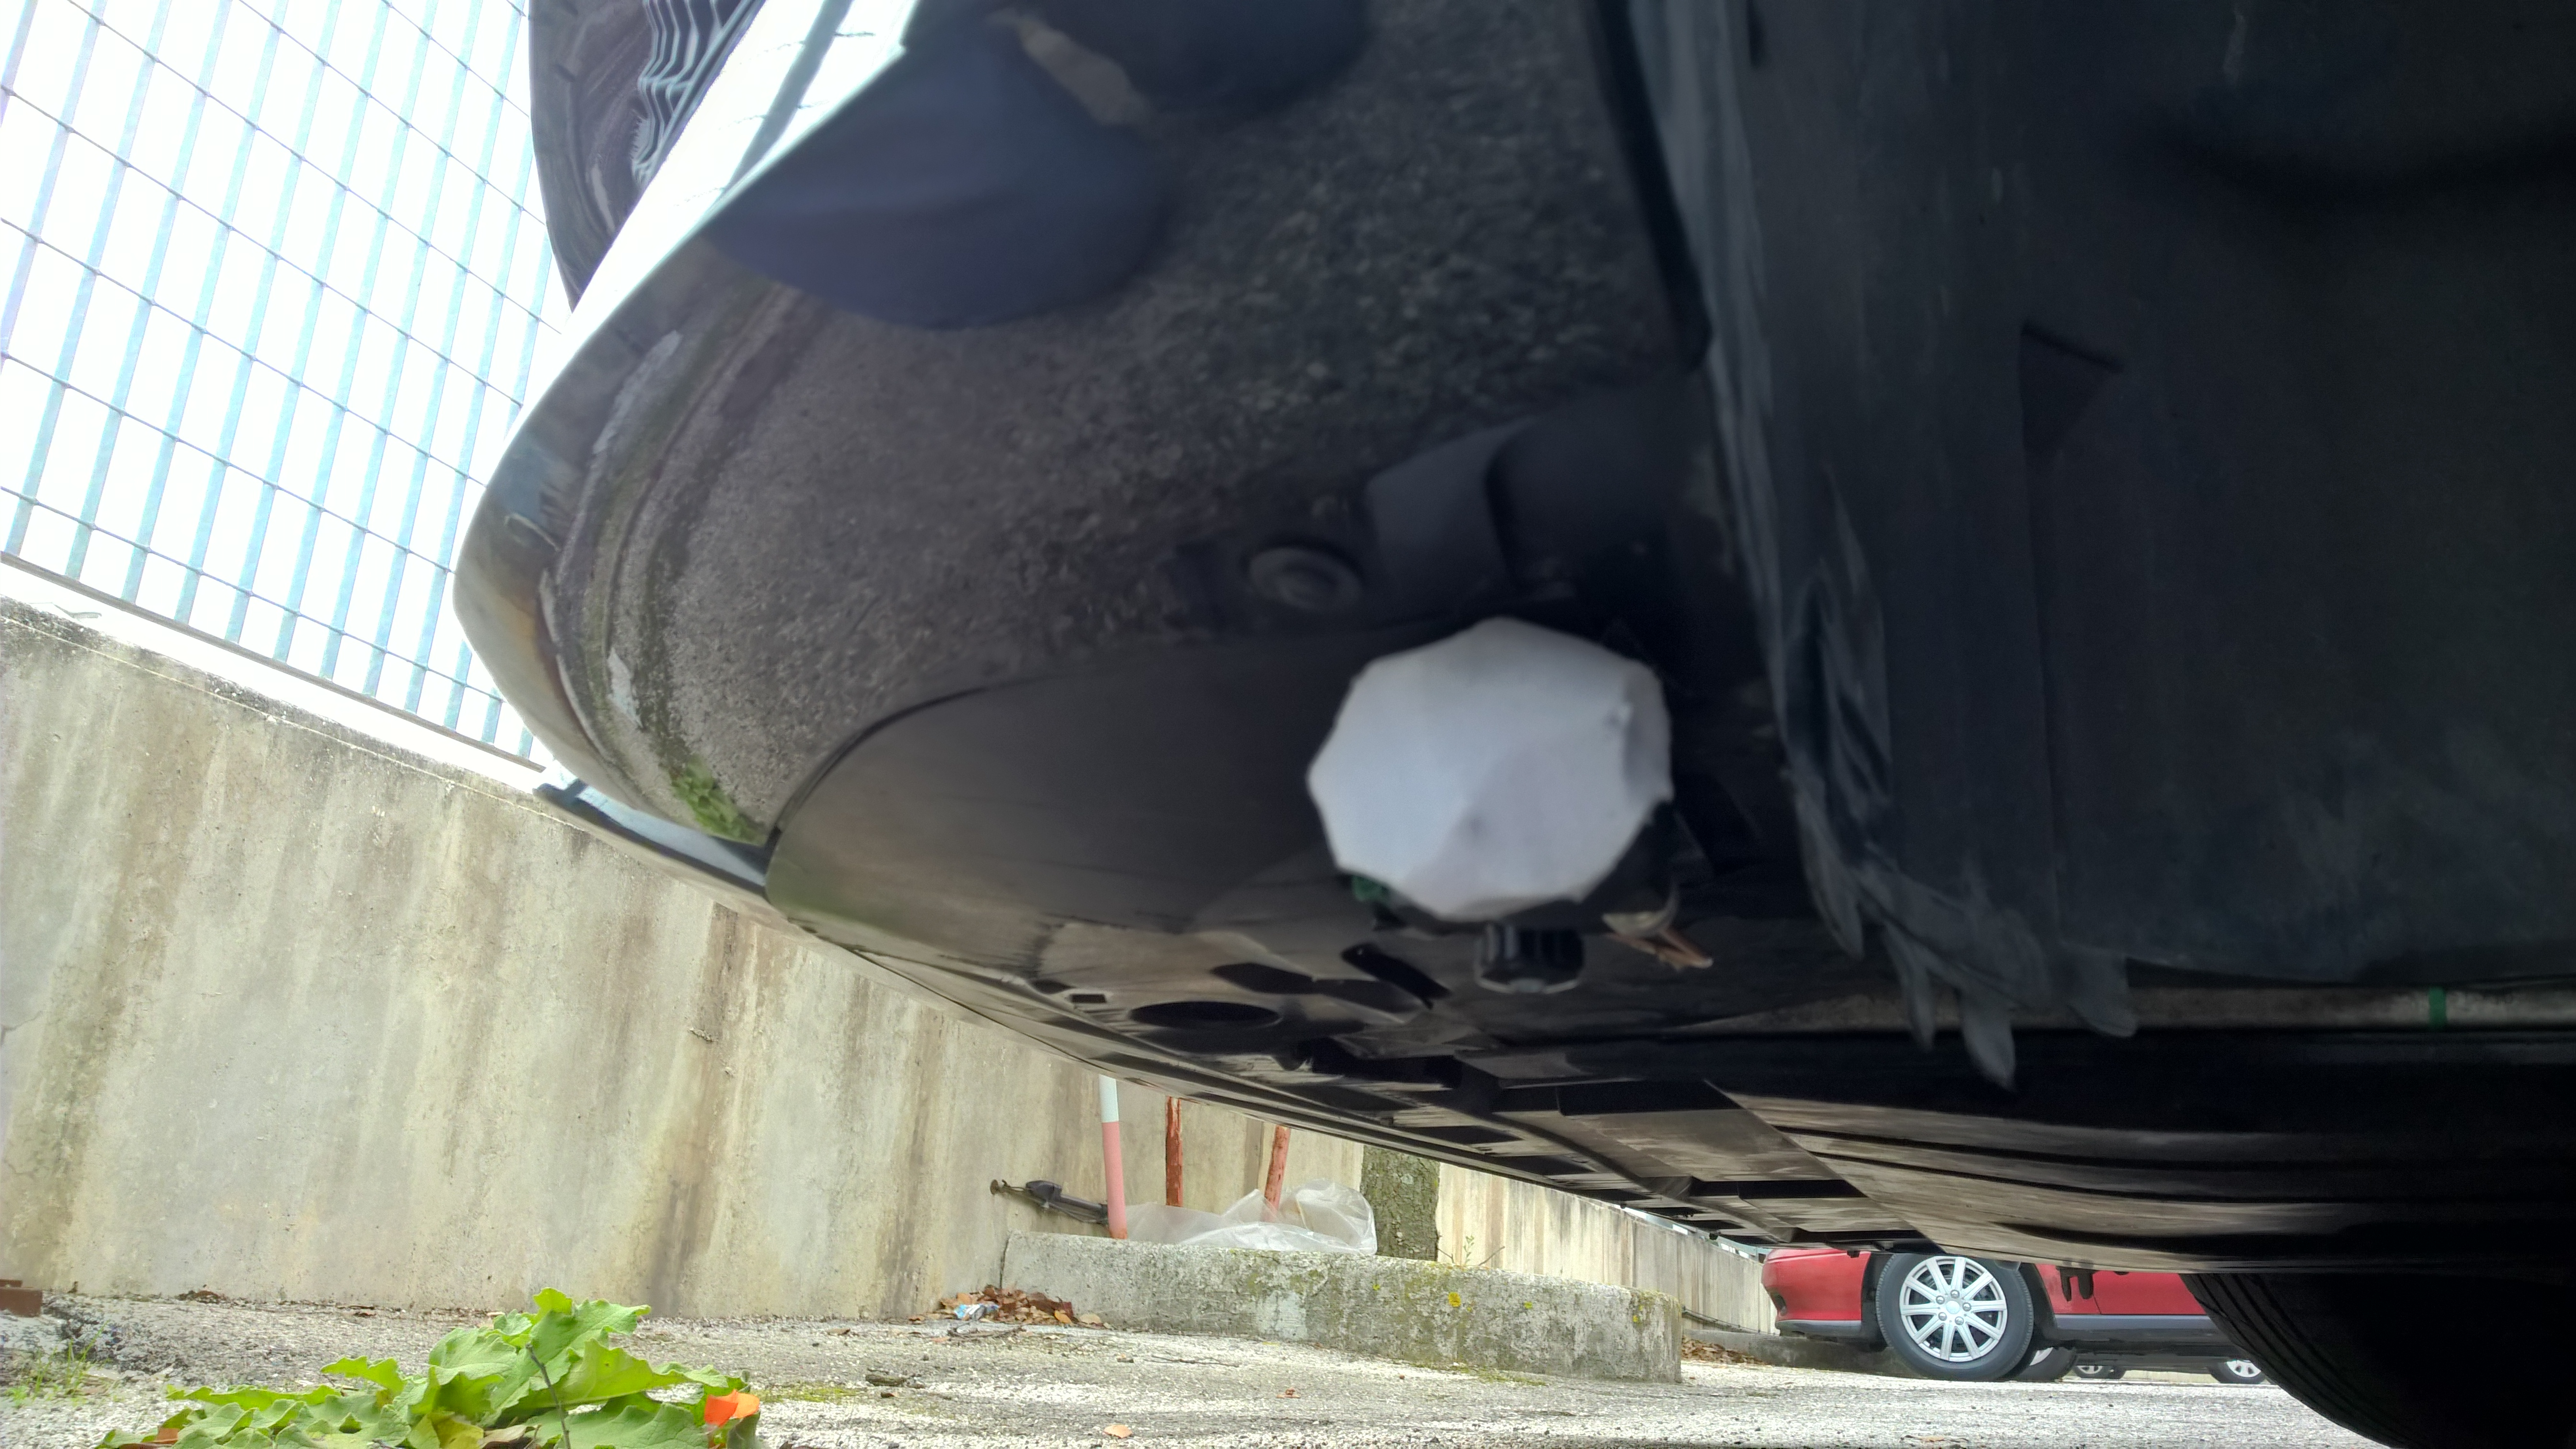
\includegraphics[width=\textwidth]{img/Front-Left.jpg}
		\subcaption{Front left tyre microphone.}
	\end{subfigure}
	
	
	\caption[\textit{PCB Piezotronics} model 130A24 microphones]{Pictures of the \textit{PCB Piezotronics} model 130A24 microphones positioned near the rear right and front left tyres, according to "RR" and "FL" red circles in \figref{fig:car-mic}. The microphones are enclosed by a melamine resin foam with open cell network structure to reduce the wind noise.}
	\label{fig:car-rr-and-fl}
\end{figure}



The car employed to build the dataset is Mercedes A Class from 2014. In addition to the audio signals, the GPS signal has been recorded to track down the car speed and position at any given time. A mobile multi-channel front end, \textit{HEAD Acoustics SQuadriga II}, has been employed as acquisition device, being able to monitor and record 8 contemporary channels at different sample rates, and to store GPS antenna and CAN bus signals.
All audio signals are sampled at 44100\,Hz, 24-bits. The external microphones used -26 dBV as input range while the interior microphones had -16 dBV as input range.
To facilitate the labelling operations, a camcorder \textit{BC Master DC10}\footnote{\url{http://www.bc-master.com/product/car-dash-camera-dc10}} was installed on the dashboard of the car. In addition to the video, it provides the speed information obtained through its own GPS antenna and it records the cockpit audio, useful for taking vocal notes while driving.

The data recorded with the \textit{HEAD Acoustics SQuadriga II} have been exported by means of the software \textit{HEAD Acoustics ArtemiS SUITE} in the uncompressed WAV audio format with a 32-bit float representation.

All recordings were taken in dry conditions in the urban and suburban areas of Ancona (Italy) with variable speed, traffic conditions and pavement roughness. Only roads that had been recently asphalted were considered and multiple takes at different speed for each road have been performed. The dataset is not perfectly balanced and is characterized by 41\% of rough road samples and 59\% of smooth road samples. For this reason a balanced version of the dataset, i.e. with equal number of smooth and rough samples, has been created by pruning excess samples for the most populated class. 
The result of the recording sessions is a 50-minutes-long dataset (41 minutes for the balanced version), with 6 audio channels and a speed channel. Labels for the roads have been annotated manually.

The spectrograms from two audio samples belonging to the smooth and rough classes are shown in Figure \ref{fig:spectrograms_road}.

\begin{figure}[ht]
	\centering
	\begin{subfigure}[b]{0.48\textwidth}
		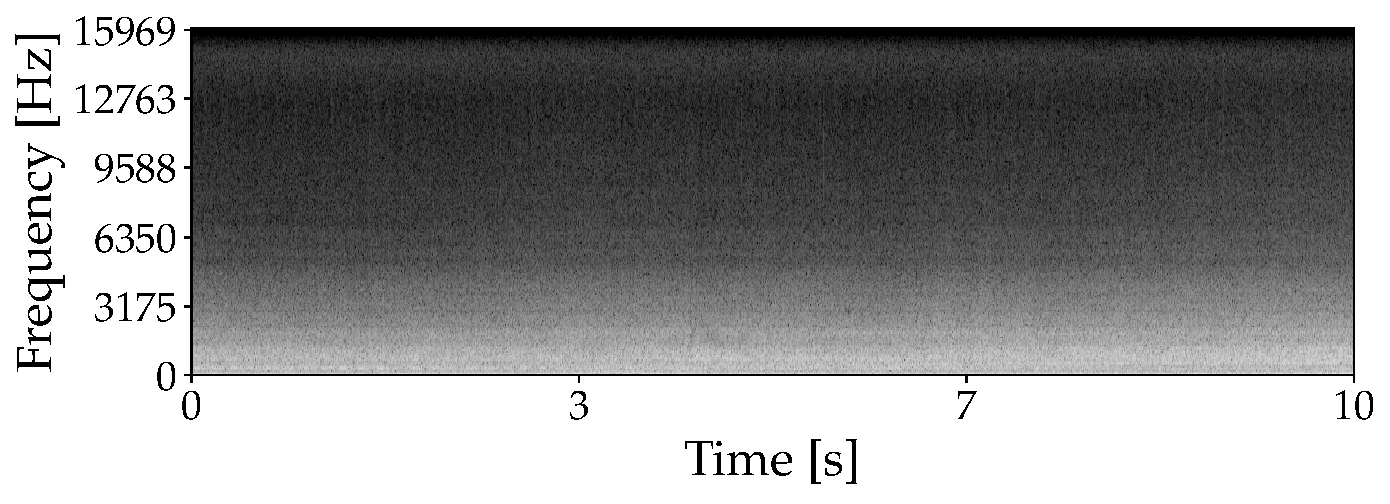
\includegraphics[width=\textwidth]{img/specgram_REC007}
		\subcaption{Smooth road.}
	\end{subfigure}
	\hfil
	\begin{subfigure}[b]{0.48\textwidth}
		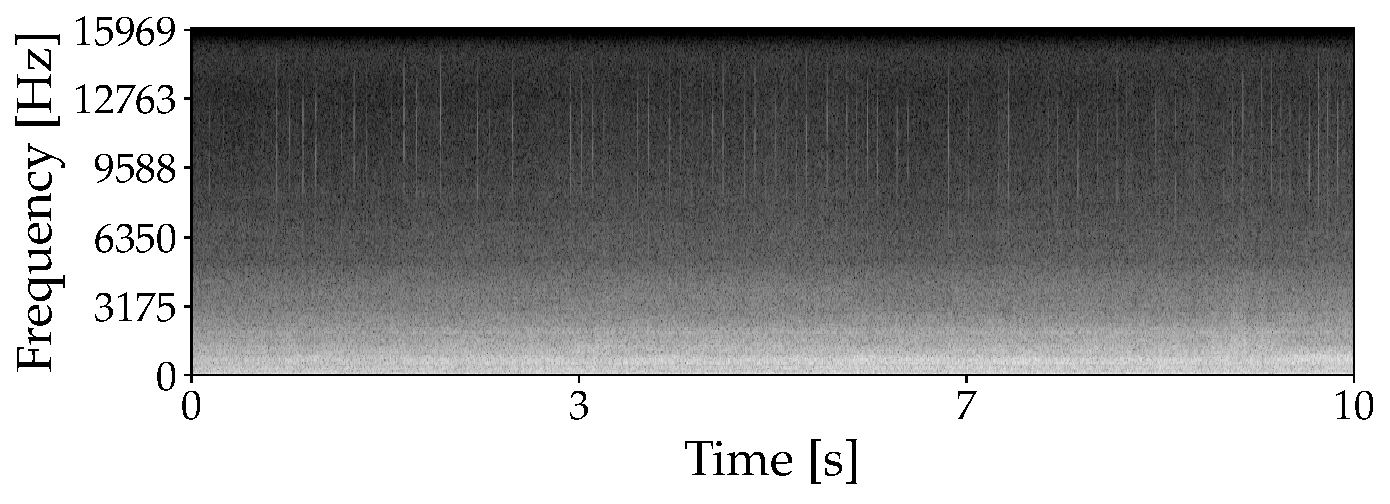
\includegraphics[width=\textwidth]{img/specgram_REC015}
		\subcaption{Rough road.}
	\end{subfigure}
	
	
	\caption[Spectrograms from 10 second samples]{Spectrograms from 10 second samples of (a) smooth urban road, (b) rough highway asphalt.}
	\label{fig:spectrograms_road}
\end{figure}

\subsection{Classification of Snore Sounds Excitation Locations}

\section{The MPSSC dataset}
\label{section:dataset}
The MPSSC dataset is composed of more than 30 hours of audio recordings captured during DISE examinations of 224 subjects from three medical centers recorded between 2006 and 2015. Recording equipment, microphone type, and location differ among the medical centers, so do the background noise characteristics. From the original signals (raw PCM, sample rate 16\,000\,Hz, quantization 16 bit) 843 early identifiable, single site of vibration snore events have been extracted and manually screened from medical experts.
Following the 4-class VOTE scheme, each sound file in the dataset is labelled as V, O, T, E, depending on the tissue from which snore sound originates, as shown in \figref{fig:vote}. They are respectively:
\begin{itemize}
	\item (V) - Velum (palate), including soft palate, uvula, lateral
	velopharyngeal walls;
	\item (O) - Oropharyngeal lateral walls, including palatine tonsils;
	\item (T) - Tongue, including tongue base and airway posterior to the tongue base;
	\item (E) - Epiglottis.
\end{itemize}

\begin{figure}[t]
	\centering
	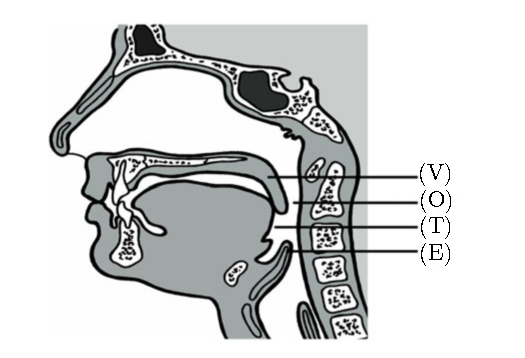
\includegraphics[width=0.6\linewidth]{img/vote.pdf}
	\caption[VOTE positions]{Corresponding positions of the VOTE classification in the upper airway. Picture courtesy of \cite{janott2014akustical}.} 
	\label{fig:vote}
\end{figure}


The dataset is divided into three subsets: \textit{train}, \textit{devel} and \textit{test}.
The number of events per class in the database is strongly unbalanced with a high preeminence of the ``Velum'' (V)-class  and ``Oropharyngeal'' (O)-class (85\% of samples) but in line with the likelihood of occurrence during normal sleep, while 10\% and 5\% of samples respectively belongs to E-events and T-snores. Details of class occurrences are shown in Table I.

\begin{table}[t]
	\centering
	\begin{tabular}{cccc}
		\toprule
		\multicolumn{4}{c}{\textbf{The Munich-Passau Snore Sound Corpus}} \\
		\midrule
		\#  \rule{10pt}{0pt}	& train  \rule{10pt}{0pt} & devel & test\\
		\midrule
		V \rule{10pt}{0pt}	& 168  \rule{15pt}{0pt} & 161 & 155\\
		O \rule{10pt}{0pt}	& 76  \rule{15pt}{0pt} & 75 & 65\\
		T \rule{10pt}{0pt}	& 8  \rule{15pt}{0pt} & 15 & 16\\
		E \rule{10pt}{0pt}	& 30  \rule{15pt}{0pt}& 32 & 27\\
		\bottomrule
		$\Sigma$  \rule{10pt}{0pt} & 282  \rule{13pt}{0pt} & 283 & 263\\
	\end{tabular}
	\caption[The Munich-Passau Snore Sound Corpus]{The Munich-Passau Snore Sound Corpus - The table shows the number of events per class in train, devel and test.}
	\label{tab:mpssc} 
\end{table}

%\begin{figure*}[t]
%	\centering
%	\includegraphics[width=\linewidth]{imgs/spectr-vote.png}
%	\caption{Waveforms and spectrograms of VOTE events}{(a) V (velum); (b) O (oropharyngeal); (c) T (tongue base); (d) E (epiglottis). \textbf{Rifare in HD, eventualmente aggiungere SCAT plot}} 
%	\label{fig:spectrograms}
%\end{figure*}


\begin{figure*}[t]
	\centering
	\begin{subfigure}{.40\textwidth}		
		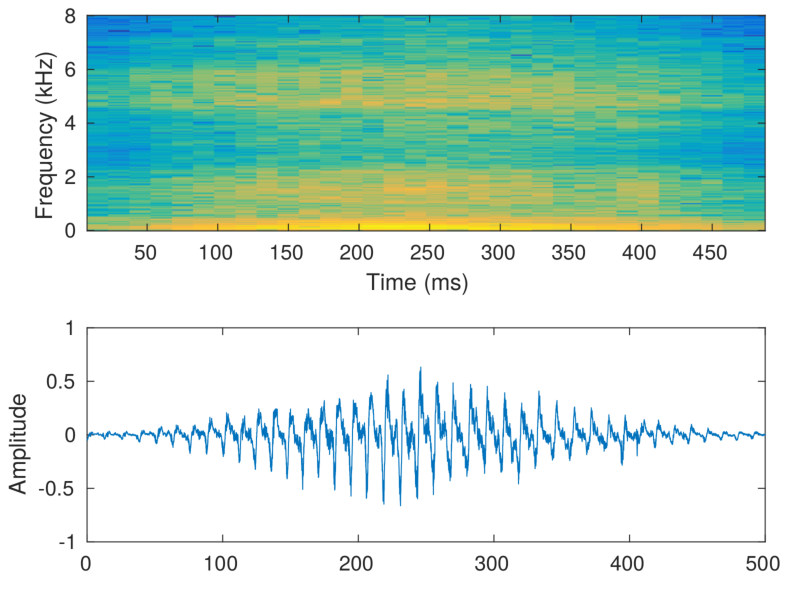
\includegraphics[width=0.9\linewidth]{img/V_spec_crop.pdf}
		\caption{}
		\label{fig:V}
	\end{subfigure}
	\begin{subfigure}{.4\textwidth}
		%\centering
		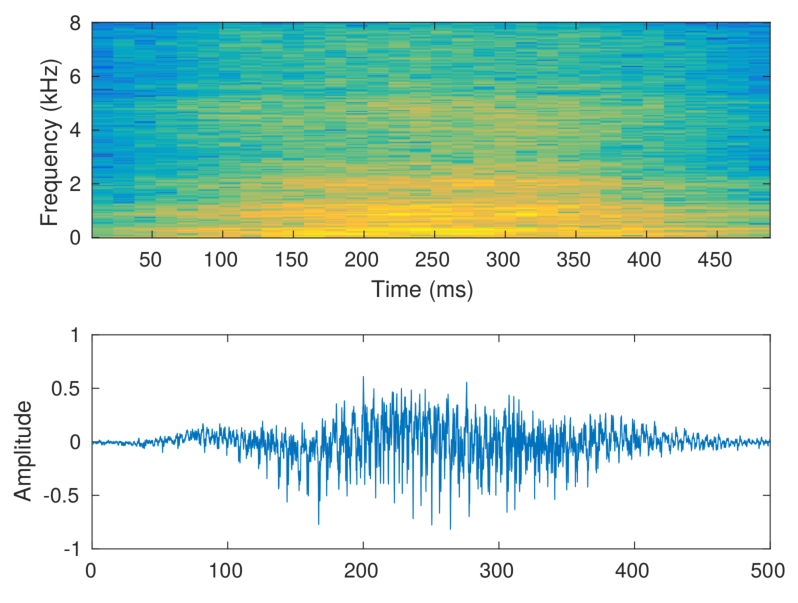
\includegraphics[width=0.9\linewidth]{img/O_spec_crop.pdf}
		\caption{}
		\label{fig:O}
	\end{subfigure}
	\begin{subfigure}{.40\textwidth}
		%\centering
		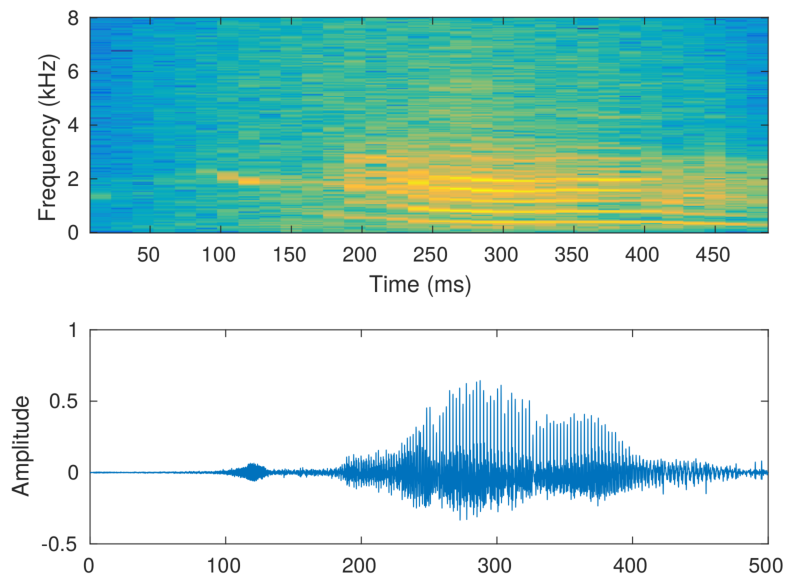
\includegraphics[width=0.9\linewidth]{img/T_spec_crop.pdf}
		\caption{}
		\label{fig:T}
	\end{subfigure}
	\begin{subfigure}{.40\textwidth}
		%\centering
		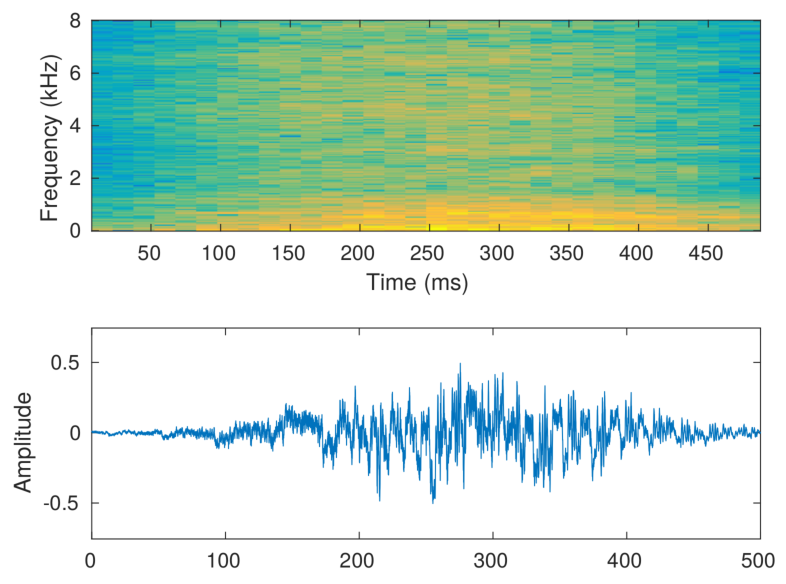
\includegraphics[width=0.9\linewidth]{img/E_spec_crop.pdf}
		\caption{}
		\label{fig:E}
	\end{subfigure}
	\caption{Waveforms and spectrograms of VOTE events}{(a) V (velum); (b) O (oropharyngeal); (c) T (tongue base); (d) E (epiglottis).}
	%\caption{Scat spectrum of VOTE events.  The top image is made of first-order coefficients, organized in a time-scale matrix. at the bottom of the image appear very low frequencies. The second-order coefficients for a fixed scale $m_1$, are shown in the bottom image, again in a time-scale matrix.}{(a) V (velum); (b) O (oropharyngeal); (c) T (tongue base); (d) E (epiglottis).}
	\label{fig:spectrograms}
\end{figure*}
As shown in the waveforms and the related spectrograms in \figref{fig:spectrograms}, the main energy components in three of the classes are concentrated in the frequency area below around 2000 Hz. Energy and spectral distribution characteristics are similar, except for the Type T, which shows higher energy content above 2500 Hz compared to the other three.


\subsection{Bird Audio Detection}
%\label{ssec:dataset}
According to the DCASE 2018 guidelines, the performance of the proposed algorithm has been assessed firstly by using the development dataset for training and validation of the system. Then, a blind test on the provided evaluation dataset was performed with the models which achieved the highest performance and submitted to the organizers of the challenge. The complete dataset is composed of recordings belonging to five different collections. Further details are reported below: %Further details are reported in Table \ref{tab:dataset}.

\begin{itemize}
	\item ``freefield1010'': a collection of 7690 excerpts from field recordings around the world;
	\item ``warblrb10k'': a crowsourced dataset recorded with the \textit{Warblr}\footnote{https://www.warblr.co.uk/} smartphone app. It covers a wide distribution of UK locations and environments and includes weather noise, traffic noise, human speech and even human bird imitations; 8000 samples are used in the development dataset while a held-out set of 2,000 recordings from the same conditions is included in the evaluation split;
	\item ``BirdVox-DCASE-20k'': 20000 files containing remote monitoring flight calls collected from  recordings units placed near Ithaca, NY, USA during the autumn of 2015;
	\item ``Chernobyl'': dataset collected from unattended remote monitoring equipment in the Chernobyl Exclusion Zone (CEZ). A totoal of 6620 audio files cover a range of birds and includes weather, large mammal and insect noise sampled across various CEZ environments, including abandoned village, grassland and forest areas;
	\item ``PolandNFC'': 4000 recordings obtained from a project of monitoring of autumn nocturnal bird migration. They were collected every night, from September to November 2016 on the Baltic Sea coast, Poland, using Song Meter SM2 units with microphones mounted on 3–5 m poles.
\end{itemize}

\begin{table}[t]
	\centering
	\begin{tabular}{|c|c|c|}
		\hline
		\ \textbf{Collection} \rule{0pt}{10pt} & \textbf{N. of samples}  & \textbf{Balance} \\
		\hline
		\hline	
		\multicolumn{3}{|c|}{\textbf{Development Dataset}  \rule{0pt}{10pt}} \\ 
		\hline
		``warblrb10k'' & 8000 & 0.75 \\
		\hline
		``BirdVox-DCASE-20k'' & 20000 & 0.5 \\
		\hline
		``freefield1010'' & 7690 & 0.25 \\
		\hline
		
		Total 	& 35690	& 0.5 \\
		
		\hline
		\hline
		
		\multicolumn{3}{|c|}{\textbf{Evaluation Dataset}  \rule{0pt}{10pt}} \\ 
		\hline
		``warblrb10k\_test'' & 2000 & - \\
		\hline
		``Chernobyl'' & 6620 & - \\
		\hline
		``PolandNFC'' & 4000 & - \\
		\hline
		Total 	& 12620 & - \\
		\hline
	\end{tabular}
	\caption{Details of the dataset we used for the algorithm development. The table shows the number of audio files and the ratio between positive/negative samples (if available) of each used data collection.}
	\label{tab:dataset} 
\end{table}

The organizers recommended a 3-way cross-validation (CV) for the algorithms development, thus in each fold we used two sets for training and the other one as validation set in order to have scores comparable with the others challenge participant.

\section{Evaluation Metrics}
\label{sec:evaluation_metrics}
Evaluation is usually referred as estimating the performance of a system under test
when confronted with new data. For an objective evaluation, the system is fed
previously unseen data for which reference annotations are available. The system output is then compared to the reference to calculate measures of its performance.

What performance means and how it should be measured may vary depending
on the specifications and requirements of the developed system: We can measure
accuracy to reflect how often the system correctly classifies or detects a sound, or we can measure error rates to reflect how often the system makes mistakes. By using
the same data and the same methodology to evaluate different systems, a fair and direct comparison can be made of systems’ capabilities.

The metrics used in detection and classification of sound events include accuracy, precision, recall, F-scor, area under the curve (AUC) or error rate (ER). There is no metric universally good for every kind of algorithm, as they each reflect different perspectives on the ability of the system.

\subsection{Metrics Computation}
Basically, the evaluation metrics are computed by comparing the prediction of the system under analysis with the respective annotations or \textit{ground truth}. Thus, the metrics are calculated based on counts of the correct predictions and different types of errors made by the system.
These counts are referred to as intermediate statistics and are defined depending on the evaluation procedure. These intermediate statistics are defined as follows for a target sound event:

\begin{itemize}
	\item True positive: A correct prediction, meaning that the system output and the reference both indicate the event present.
	\item True negative: The system output and the reference both indicate event not present.
	\item False positive: The system output indicates event  present or active, while the reference indicates event not present.
	\item False negative: The system output indicates event not present or inactive, while the reference indicatesit as present.
\end{itemize}

Sound event classification is usually a single-label multiclass problem, and the resulting intermediate metrics reflect whether the single true class is correctly recognized for each example. In this task there is no distinction between false positives and false negatives. 
In sound event detection, the choice of measurement determines the interpretation of the result: With a segment-based metric, the performance shows how well the system correctly detects the temporal regions where a sound event is
active; with an event-based metric, the performance shows how well the system is able to detect event instances with correct onset and offset. Thus, in the segment-based metric the ground truth and system output are compared in a fixed time grid, and sound events are marked as active or inactive in each segment. For the event-based metric the ground truth and system output are compared at event instance level. Specifically, the intermediate statistics for sound event detection are defined as follows:

\begin{itemize}	
	\item Substitutions $S$: are the number of ground truth events for which we have a false positive and one false negative in the same segment; %, thus: $S(t_1) = \min(FN(t_1),FP(t_1))$;	
	\item Insertions $I$: are events in system output that are not present in the ground truth, thus the false positives which cannot be counted as substitutions;%: $I(t_1) = \max(0,FN(t_1)-FP(t_1))$;
	
	\item Deletions $D$: are events in ground truth that are not correctly detected by the system, thus the false negatives which cannot be counted as substitutions;%: $D(t_1)= \max(0,FP(t_1)-FN(t_1))$.	
\end{itemize}

If we consider the scenario of polyphonic sound event detection, the segment-based metric essentially
splits the duration of the test audio into fixed length segments that have multiple associated labels, reflecting the sound events active anywhere in the given segment. In this respect, evaluation verifies if the system output and reference coincide in the assigned labels, and the length of the segment determines the temporal resolution of the evaluation. 
Event-based metrics compare event instances one to one. Since the time extents of the events detected by the system may not exactly match the ground truth, a common approach is to allow a time misalignment threshold or \textit{time-collar}.

\subsubsection{Performance Metrics}
Measures of performance are calculated based on accumulated values of the intermediate statistics. 
We denote by $TP$, $TN$, $FP$, and $FN$ the sums of the true positives, true negatives, false positives, and false negatives accumulated throughout the test data. In the case of multiclass problem, the accumulation of intermediate statistics can be performed either globally or separately for each class, depending on the nature of the problem (i.e., instance-based or class-based) or datasets characteristics (i.e., highly unbalanced classes).
Based on the total counts of the intermediate statistics, many different measures can be derived.  We can define:

\begin{eqnarray}
\text{Accuracy} =& \frac{TP+TN}{TP+TN+FP+FN} \\
\text{Precision} =& \frac{TP}{TP+FP} \\
\text{Recall} =& \frac{TP}{TP+FN}  \\
\text{F-score} =& \frac{2TP}{2TP+FN+FP}  
\end{eqnarray}

Accuracy measures how often the classifier makes the correct decision,
 as the ratio of correct system outputs to total number of outputs. Precision, recall, and F-score were introduced in the context of information retrieval. F-score can be also calculated as the harmonic mean of Precision and Recall scores:

\begin{equation}
 \text{F-score} = 2 \cdot \frac{\text{Precision}\cdot\text{Recall}}{\text{Precision}+\text{Recall}}
\end{equation}

F-score has the advantage of being a familiar and well understood metric. Its main drawback is that its value is strongly influenced by the choice of averaging and the data balance between classes: in instance-based averaging the performance
on common classes dominates, while in class-based averaging (balanced metrics) it is necessary to at least ensure presence of all classes in all folds in the test data, to avoid cases when recall is undefined.

In the case of sound event detection systems, Error Rate score is the most common evaluation metric. Considering a single time frame  $t_1$, the ER is computed from its intermediate statistics, i.e., the number of substitutions ($S(t_1)$), insertions ($I(t_1)$), deletions ($D(t_1)$) and active sound events from annotations ($N(t_1)$). Formally, for the entire evaluation set:

\begin{equation}
ER = \frac{\sum_{t_1=1}^{T} S(t_1) + \sum_{t_1=1}^{T} I(t_1) + \sum_{t_1=1}^{T} D(t_1)}{\sum_{t_1=1}^{T} N(t_1)},
\end{equation}
where $T$ is the total number of segments $t_1$.


\subsection{Detection Metrics}
Precision and recall rely on hard decisions made for each trial, they typically depend on a threshold applied to some underlying decision variable, i.e., the output of the neural network. 
Lowering the threshold will increase likelihood of accepting both positive and negative examples, improving recall but in many cases hurting precision. Although F-score combines these values at a single threshold in an attempt to balance this
tradeoff, a more complete analysis can be provided by plotting a function proportional to the metric over the full range of possible thresholds. Some examples are, the precision-recall (P-R) curve and the receiver operating characteristic (ROC) curve. The latter plots true positive rate (TPR = $TP/TP+FN$) as a function of the false
positive rate (FPR = 1 - Recall) as the decision threshold is
varied. 

These curves carry rich information, they can be difficult to compare, so a
 single figure of merit summarizing the tradeoff is desirable. The
relative ``compressed'' scores for P-R and ROC curve are respectively Average Precision (AP) score
or Area under curve (AUC), defined as:

\begin{equation}
\text{AP} = \sum_n (R_n-R_{n-1})P_n,
\end{equation}
where $R_n$ and $P_n$ are the Recall and Precision for threshold $n$ respectively and
\begin{equation}
\text{AUC}=\int _{\infty }^{-\infty }{\mbox{TPR}}(T){\mbox{FPR}}'(T)\,dT
\end{equation}
Both AUC and AP vary between 0 and 1, with an uninformative classifier yielding 0.5, while the ideal system yelds 1.


\subsection{Final Remarks}
Estimates of metrics on classes with very few examples are also intrinsically noisy. Any dataset of real-world
recordings will most likely have unbalanced event classes; therefore, the experiment setup must be built with the choice of metric in mind. In a cross-validation approach, a more stable result is given by treating the cross-validation folds as single experiment, meaning that metrics are calculated only after training and testing all folds, not as average of the individual folds nor as average of individual class performance. In addition, reporting the variance among the individual folds’ contributions to the average
can serve as a useful confidence interval.
Anyway, if there are multiple scenes in the dataset, typically evaluation metrics are calculated for each scene separately and then the results are presented as the average across the scenes.


Attention should be also paid to statistical significance of the results and it should be used to calculate the theoretical limits of discriminability of the evaluation, especially when two methods/approaches/techniques are compared.


A detailed and visualized explanation of evaluation score in multi label setting for sound event analysis can be found in  \cite{mesaros2016metrics}.







%In this work we used the Error Rate (ER) as primary evaluation metric to ensure comparability with the reference systems. In particular, for the evaluations on the TUT-SED 2016 and 2017 datasets we consider a segment-based ER with a one-second segment length, while for the TUT-Rare 2017 the evaluation metric is event-based error rate calculated using onset-only condition with a collar of 500 ms. 
%





\chapter{Other contributions}

\section{Acoustic Novelty Detection with Adversarial Autoencoders}
\begin{figure}[h]
	\begin{subfigure}[t]{0.9\columnwidth}
		\def\svgwidth{0.5\columnwidth}
		% This file was created by matlab2tikz.
%
%The latest updates can be retrieved from
%  http://www.mathworks.com/matlabcentral/fileexchange/22022-matlab2tikz-matlab2tikz
%where you can also make suggestions and rate matlab2tikz.
%


\begin{tikzpicture}

\begin{axis}[%
width=0.85\columnwidth,
height=4cm,
at={(1.424in,0.703in)},
scale only axis,
point meta min=-156.535576728001,
point meta max=-22.4028070325664,
axis on top,
xmin=0.008,
xmax=29.992,
ytick={0,1,...,8},
x label style={at={(axis description cs:0.50,-0.06)},anchor=north},
y label style={at={(axis description cs:0.0,0.4)},anchor=south},
xlabel style={font=\color{white!15!black}},
xlabel={Time (s)},
ymin=-0.015625,
ymax=8.015625,
ylabel style={font=\color{white!15!black}},
ylabel={Frequency (kHz)},
axis background/.style={fill=white},
colormap/jet
%colorbar,
%colorbar style={ylabel style={font=\color{white!15!black}}, ylabel={Power/frequency (dB/Hz)}}
]
\addplot [forget plot] graphics [xmin=0.008, xmax=29.992, ymin=-0.015625, ymax=8.015625] {img/spectrogram-1_highlight.png};
%\draw[black,line width=2pt] (axis cs:4.7,4) ellipse (12 and 400);

%\draw[line width=1.2pt](axis cs:3.65,8) rectangle (axis cs:5.7,0);

%\node [draw, ellipse, thick, red, minimum width=14, minimum height=200, label=above:Novelty] at (axis cs:4.7,4) {};
\node[text=white] at (axis cs:4.7,4)[rotate=90] {\contour{white}{Novelty}};

%\draw[black,line width=2pt] (axis cs:18.5,4) ellipse (12 and 400);
%\draw[line width=1.2pt](axis cs:17.5,8) rectangle (axis cs:19.55,0);
\node[text=white] at (axis cs:11.6,4)[rotate=90] {\contour{white}{Novelty}};

%\draw[black,line width=2pt] (axis cs:25,0.5) ellipse (50 and 40);
%\draw[line width=1.2pt](axis cs:20,5) rectangle (axis cs:29.95,0);

%\fill[black, opacity=0.4](axis cs:20,5) rectangle (axis cs:29.95,0);
%\fill[white, opacity=0.5](axis cs:22,3) rectangle (axis cs:28.00,1);

\node[text=white] at (axis cs:25,4) {\contour{white}{Normal}};



\end{axis}
\end{tikzpicture}%
	\end{subfigure}	
	\caption[Acoustic Novelty Detection]{Spectrogram of an audio signal with novel and normal data.}
\end{figure}
Novelty detection is the task of recognising events the differ from a model of normality. This paper proposes an acoustic novelty detector based on neural networks trained with an adversarial training strategy. The proposed approach is composed of a feature extraction stage that calculates Log-Mel spectral features from the input signal. Then, an autoencoder network, trained on a corpus of ``normal'' acoustic signals, is employed to detect whether a segment contains an abnormal event or not. A novelty is detected if the Euclidean distance between the input and the output of the autoencoder exceeds a certain threshold. The innovative contribution of the proposed approach resides in the training procedure of the autoencoder network: instead of using the conventional training procedure that minimises only the Minimum Mean Squared Error loss function, here we adopt an adversarial strategy, where a discriminator network is trained to distinguish between the output of the autoencoder and data sampled from the training corpus. The autoencoder, then, is trained also by using the binary cross-entropy loss calculated at the output of the discriminator network.  

The performance of the algorithm has been assessed on a corpus derived from the PASCAL CHiME dataset. The results showed that the proposed approach provides an F1-score equal to 93.28\%, with a relative performance improvement equal to 0.26\% compared to the standard autoencoder. The significance of the improvement has been evaluated with a one-tailed z-test and resulted significant with $p<0.001$. The presented approach thus showed promising results on this task and it could be extended as a general training strategy for autoencoders if confirmed by additional experiments.

\subsection{Details}
In this work, we are not interested in the generative capabilities of the network, since in the novelty detection task the objective is to minimise the error made by the autoencoder in reconstructing normal data. Thus, the architecture and the training strategy are different from \cite{makhzani2015adversarial}: the discriminator network is trained to discriminate between data from a training set and data reconstructed by the autoencoder (\figref{fig:our_training}). The final layer of the discriminator is a single neuron with sigmoid activation function and its output represents the probability of the data of being sampled from the training set. At the end of the training phase, the discriminator network should not be able to distinguish training set data and reconstructed data, i.e., its output should be constantly equal to 0.5.

Similarly to \cite{goodfellow2014generative}, the training process can be viewed as a min-max game between the autoencoder and the discriminator network. Let $\boldsymbol{x}$ be an input feature vector, $\tilde{\boldsymbol{x}} = A(\boldsymbol{x})$ the output of the autoencoder, and $D(\boldsymbol{x})$ the output of the discriminator network, i.e., the probability of $\boldsymbol{x}$ of being sampled from the training data. The training procedure is composed of three main phases: the first phase and the third phase consist in updating the autoencoder and the discriminator respectively by minimising the reconstruction error and the classification error (binary cross-entropy). The middle phase incorporates the interaction between the two networks: the autoencoder weights are updated based on the output the discriminator network.


Whether a feature vector is a novel sound or a normal background sound is determined by calculating the reconstruction error, i.e., the Euclidean distance between the output produced by the autoencoder and the input data itself. If the distance exceeds a predefined threshold, the input data is classified as novelty, otherwise as normal. The threshold is calculated as follows: for each input sequence the threshold $\theta$ is calculated with the following expression:
\begin{equation}
\theta = \beta \cdot \text{median}\{e(1),\ldots,e(N)\},
\end{equation}
where $e(i)$ is reconstruction error of feature vector $i$ in the signal, $N$ is the number of features, and $\beta \in [1, 2]$ is a predefined constant.

\begin{figure}[h]
	\centering
	\begin{subfigure}[t]{0.7\columnwidth}
		\def\svgwidth{\columnwidth}
		\input{7_other_contributions/img/our_approach.pdf_tex}
		
		\caption{Proposed architecture for training an autoencoder with an adversarial discriminator network.}\label{fig:our_training}
	\end{subfigure}
	\par\bigskip
	\begin{subfigure}[t]{0.7\columnwidth}
		\def\svgwidth{\columnwidth}
		\input{7_other_contributions/img/detection.pdf_tex}
		
		\caption{Novelty detection phase.}\label{fig:our_detect}
	\end{subfigure}
	\caption[Acoustic Novelty Detection with GANs]{The proposed approach for novelty detection with adversarial autoencoders. For the sake of simplicity, the feature extraction stage is not shown.}\label{fig:approach}
\end{figure}

\newpage
\section[Siamese Nets for Human-Fall Detection]{Few-shot Siamese Neural Networks employing Audio features for Human-Fall Detection}

Nowadays, the detection of human fall is a problem recognized by the entire scientific community. Methods that have good performance use human falls samples in the train set, while methods that do not use it, can only work well under certain conditions. Since examples of human falls are very difficult to retrieve, there is a strong need to develop systems that can work well event with few or no data to be used for their training phase. In this work, we show a first study on few-shot learning Siamese Neural Network applied to human falls detection by using audio signals. This method has been compared with algorithms based on SVM and OCSVM, all evaluated starting from the same conditions. The proposed approach is able to learn the differences between signals belonging to different classes of events. In classification phase, using only one human fall signal as a template, it achieves about 80\% of  $ F_1 -Measure$ related to the human fall class, while the SVM based method gets around 69\%, when it is trained in the same data knowledge conditions.

\subsection{Proposed Approach}

In this work we propose a Siamese Neural Network able to learn a latent representation of an audio event. In particular, a SNN is composed of two twin networks with binded weights. A pair of inputs is provided to the system, one to each twin network. Downstream, the network maps these inputs into two different representation vectors. Then, a certain type of distance between those two representations is computed. In this work euclidean distance was used. In \figref{proposed_approach}, are reported two example of mel-spectrograms: the spectrum that is given as input to the function first network represents a chair that is overturned. The other inputs instead represent a human fall. As can be seen, the signals are not distinguishable at a glance, thus we think that the differential approach of the SNN, described below, seems to be appropriate.

Our Siamese network has been trained on a corpus of labelled object fall events and not including any human fall. Pairs of events belonging to the same class correspond to the positive examples while pairs of events belonging to the different class a negative one. In particular, the term few-shot comes from the fact that although, in this case study, human falls have not been used for training, some of them are used in the optimization phase, before the final test.
\begin{figure}
	\centering
	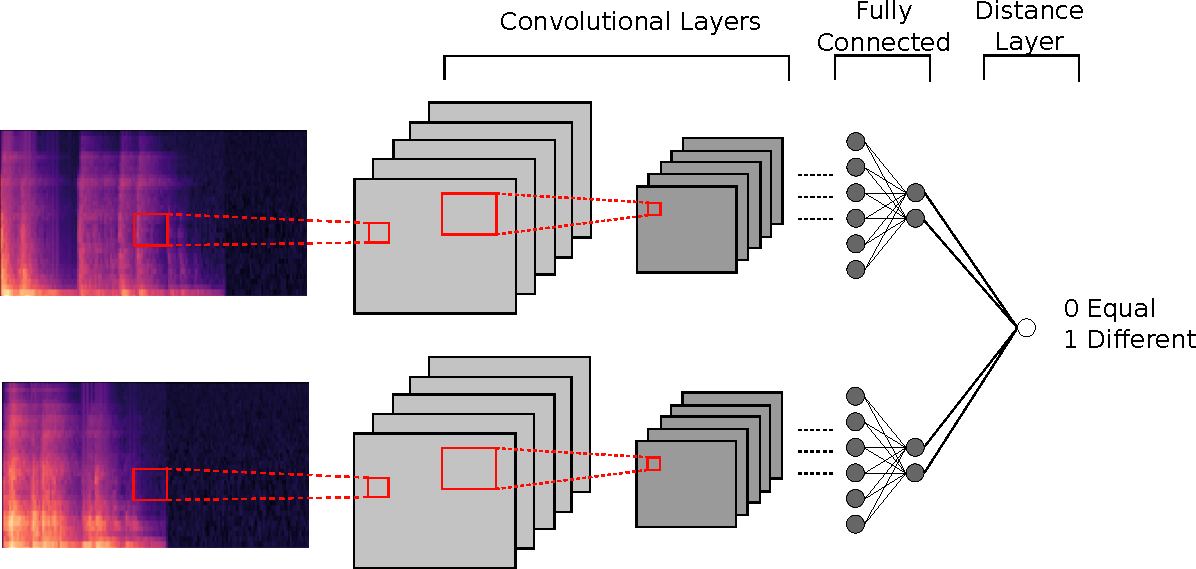
\includegraphics[width=0.7\linewidth]{img/Siamese_approach}
	\caption[Siamese Nets for Human-Fall Detection]{Proposed approach for Human-Fall Detection.}
	\label{proposed_approach}
\end{figure}

\subsection{Results}
The results obtained for each method are reported in \figref{fig:results_f1}. The figure shows the $ F_1 -Measure$, false negative rate (miss rate) and false positive rate (false alarm rate) referred to the human fall class. It is clear that the supervised SVM method outperforms all other in terms of  $ F_1 -Measure$ as expected. The OCSVM instead is the worst method if used in this context, because its training procedure does not include any human fall, but the normality model is composed of others types of falls, making it difficult to identify the human fall as ``novelty''. The Siamese and the SVM-unbalanced, which start from the same data for the training, are classified in the intermediate positions as expected. However, we note that the proposed approach achieves a better result, exceeding the $ F_1 -Measure$ of SVM-unbalanced of about 11\%. 

\begin{figure}[h]
	\centering
	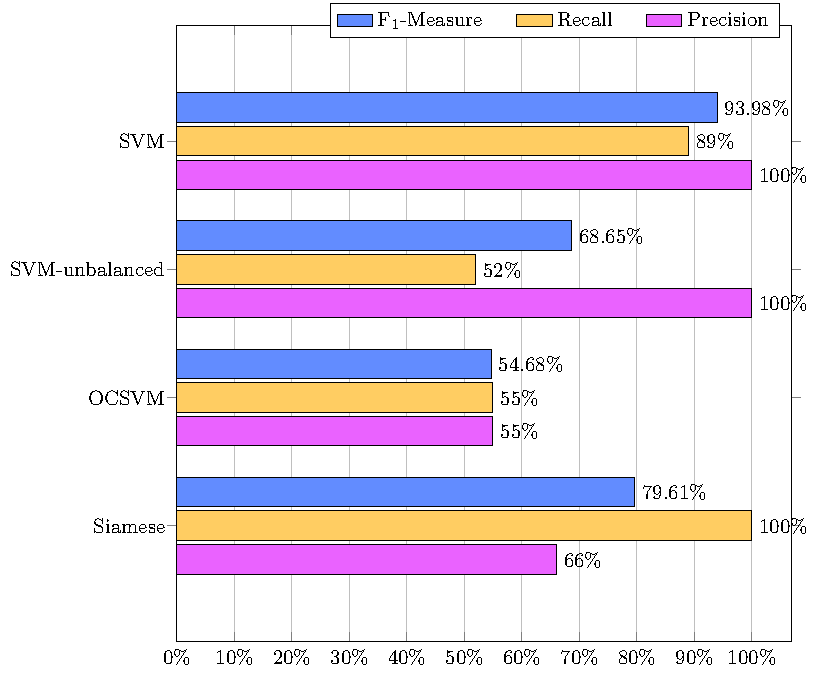
\includegraphics[width=0.65\linewidth]{img/results_f1}
	\caption[Siamese Nets for Human-Fall Detection - Results]{$F_1 -Measure$, precision and recall: the metrics are referred to the human fall class}
	\label{fig:results_f1}
\end{figure}


\newpage
%%%%%%%%%%%%%%%%%%%%%%%%%%%%%%%%%%%%%%%%%%%%%%%%%%%%%%%%%%%%%%%%%%%%%%%%%%%%%%%%%%%%%%%%%%%%%%%%%%%%%%%%%%

\section{Generative Raw Audio Synthesis}
Biologically-inspired algorithms such as artificial neural networks have been used extensively by computer music researchers, for generative music and algorithmic composition. The recent introduction of raw audio Machine Learning (ML) techniques, however, represents a significant leap because they seem to be able to learn both high-level (event) and low-level (timbre) information at once. Employing such techniques for creative purposes is very challenging at this early stage since there is lack of method, experience, and their computational cost is very high. 

To the best of our knowledge, three main architectures have been proposed to learn and reproduce features from raw audio signals, namely WaveNet \cite{van2016wavenet}, sampleRNN \cite{mehri2016samplernn}, and WaveGan \cite{donahue2018synthesizing}. Recently, another architecture, named FFTnet, has been proposed \cite{jin2018fftnet} that draws some concepts from WaveNet but shows a lower computational cost. 

These architectures show the ability of learning features from raw audio data and generate similar signals drawing from a \textit{latent} representation of these data directly in the time domain. This seems to be possible thanks to a hierarchical representation of the signal. In other words, architectures such as sampleRNN and WaveNet process the signal at multiple levels, enabling the network to store significant features from the micro-scale (sample level) up to the macro-scale (1 second and more). Experiments with these two architectures show that after training the network with a few hours of piano music, the networks are able to reproduce piano tones in a somewhat organized way. They are, thus, able to learn the timbre of the piano, the piano tone envelope (attack and decay), and finally, they learn that piano notes have rhythmical patterns, can be played in clusters, chords and sequences.

Stemming from these results, the authors decided to explore the possibility of running these algorithms for tone generation. At the time of writing, these algorithms are not suitable for synthesis from a score. However, they have the autonomous ability of generating a sequence of sounds, similarly to generative algorithms, but working at several time scales.

\subsection{Algorithm Selection}\label{subsec:algorithm}

A careful evaluation of currently available machine learning algorithms for raw-audio generation has been carried on. The evaluated algorithms were:
\begin{itemize}
	\item WaveNet \cite{van2016wavenet},
	\item sampleRNN \cite{mehri2016samplernn},
	\item WaveGAN \cite{donahue2018synthesizing}.
\end{itemize}

At the time of setting up the experiments the FFTNet algorithm \cite{jin2018fftnet} was not yet published.

The WaveNet architecture allows for modeling complex data such as music and speech. It is based on a stack of causal dilated convolutional layers for feature extraction. The dilated convolutions are key to extract features at different levels (closely resemblant to a dyadic wavelet filter bank \cite{jin2018fftnet}), however, the experiments in \cite{cabello2017autoregressive} show that the use of dilated convolutions alone do not allow modelling complex raw audio sequences, thus, residual blocks and the use of skip connections after the convolutional layers are necessary to speed up convergence and allow the training of a deep model. The ability of the network to model meaningful sequences of samples relies on causal probability conditioning, i.e. the last output sample is conditioned by the probability of all previous output samples. Additionally, it has been shown with speech synthesis that the output sample probability can be conditioned with, e.g. speaker timbre and phonemes. In our case, however, we are not interested in leveraging this feature, leaving the network to generate freely.

The main issue preventing adoption of WaveNet is its high computational cost and informal reports of their performance seems to confirm this. To test the feasibility of the approach and verify these claims we adapted one of the several open-source implementations of WaveNet currently available. We conducted preliminary experiments on a Titan X GPU employing Theano as backend. After 72 hours of training using the same piano dataset suggested by \cite{van2016wavenet} the network was still unable to provide results vaguely similar to the ones shown by the authors of \cite{van2016wavenet}. Furthermore, some of the hyperparameters were extrapolated from the paper, but most of them are not available, so a hyperparameters search would be required, increasing the training times far over our available resources.

A very different approach is followed by the authors of sampleRNN \cite{mehri2016samplernn}. This architecture is based on the same principle of causal probability conditioning, however, in this case the network consists of several tiers of recurrent neural networks (RNN) working at different temporal resolutions. Each RNN conditions the RNN at the lower tier. SampleRNN has been tested with both speech and music database. Both database are a few hours long.

We also performed preliminary experiments employing the open-source implementation provided by the authors of \cite{mehri2016samplernn} on the same hardware reported above. This implementation is based on Theano and Lasagne. Results are on par with those provided by the authors and training times can have length of 1-4 days depending on the input material and the degree of fitness that is required.

Finally, we considered WaveGAN for sound generation. This architecture is based on the generative adversarial networks (GAN) paradigm. The authors of \cite{donahue2018synthesizing} devised two models, WaveGAN, working on the raw audio with 1D convolutions and SpecGAN, working with 2D spectrograms. The outcomes of their work are very promising, since these two architecture are able to learn from a much shorter database than WaveNet and sampleRNN. However, they are inherently designed to synthesized audio of a specific length (16384 samples for WaveGAN or a 128x128 spectrogram for SpecGAN). For this reason they are not well suited for generative audio. Running a WaveGAN several times would introduce issues in concatenating each output.

At the end of this evaluation stage, we decided to use sampleRNN. 


\subsection{Input Material and Dataset Creation}\label{subsec:input}

The input material for this work has been provided by artist \textit{\O kapi} in form of \textit{stems} of his musical project Rima Glottidis. The main goal of the work was to generate vocal textures from his material to be arranged in form of a site-specific sound installation. The stems came from cut recordings of male and female speech of several speakers showing proper Italian pronunciation vs. unclear spelling and regional accent.

Additionally they presented bell tones, singing choirs, sung phonemes, and silence, revealing part of the musical structure of the original project. The whole material length was 14 minutes. A subset of this material, totalling 7 minutes, was obtained by leaving only the speaking voices and cutting all other musical material.

From previous experience with sampleRNN the input material was judged to be too short. Informal experiments on voice synthesis were conducted in 2016 by the first author showing that sampleRNN can faithfully learn the vocal timbre of a speaker only from a sufficiently large and homogeneous dataset of speech. Specifically, a 3 hours dataset gathered from publicly available speeches of a well known Italian comedian and politician was used to train a three-tier sampleRNN model. At the end of the training, a convincing babbling was obtained with random phonemes. Most subjects presented with the synthesized speech could recognize the identity of the public figure. Reducing the dimension of the dataset to 1 hour or less degraded the performance of the network making the utterances noise-like.

To increase the chances to obtain interesting audio material from sampleRNN, other audio material has been selected. Data augmentation has been tested to enlarge the training corpus without adding spurious material that would reduce the portion of material from \textit{\O kapi}. Data augmentation has been done by pitch shifting audio data by -3 and +3 semitones. 

Additionally, 22 minutes of choral works from Arvo P\"art were added. A subset of this dataset has been randomly selected, totalling 2 minutes. These datasets have been used for training 2 different sampleRNN models with hyperparameters suggested by the authors of \cite{mehri2016samplernn}. Training of these models was conducted with a Titan X GPU and left running for 2 days for each one, approximately lasting for 220 epochs (approx $3 \cdot 10^6$ iterations). For each epoch, several 10s-long pieces of randomly generated material were extracted for later use. 

\subsection{Results}
Discussion about the network outcomes will be qualitative, as there is no objective means to assess the quality of the material. The loss employed by sampleRNN, the categorical crossentropy, does not clearly state the quality of the sound material. The largest excursion of the loss seen during training ranged from 5 to 3 for the training set and from 4.5 to 3.9 for the validation set. Notwithstanding this, the first tones generated were pure noise, while the last ones had some of the character of the original dataset. The training loss did not necessarily decrease with time and samples with interesting features emerged at different epochs. Most notably, samples generated at a given epoch or at consecutive epochs, have all very similar features that later disappear with the training.

The outcomes from these trainings can be divided in several classes: speech-like babbling (a), whistling (b), rumbles and impulses (c) or mixtures of the above. Figure \ref{fig:esempi} shows spectrograms of each class. Please note that the whistling tones do not appear in the output generated from the Rima Glottidis speech-only subset. It was noted, indeed, that these have the same frequency of bell tones found in the complete Rima Glottidis dataset. Bell tones appear on the 5\% of the Rima Glottidis dataset. This means that very simple and repetitive material can be easily reproduced by sampleRNN even though it does appear on a small portion of the dataset.
\begin{figure}[h]
	\centering
	%\vspace{-0.5cm}
	
	\begin{subfigure}[b]{0.45\columnwidth}
		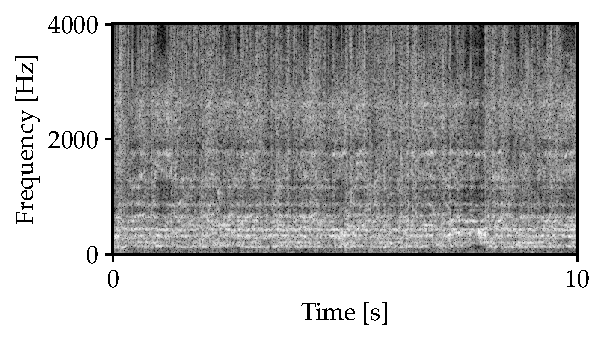
\includegraphics[width=\textwidth]{img/choral.pdf}
		\subcaption{}
	\end{subfigure}	
	\begin{subfigure}[b]{0.45\columnwidth}
		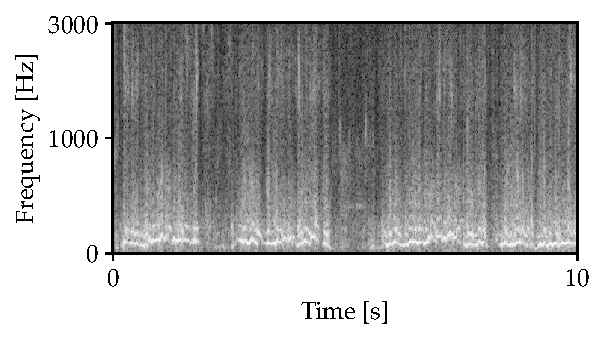
\includegraphics[width=\textwidth]{img/speech2.pdf}
		\subcaption{}
	\end{subfigure}
	
	\begin{subfigure}[b]{0.45\columnwidth}
		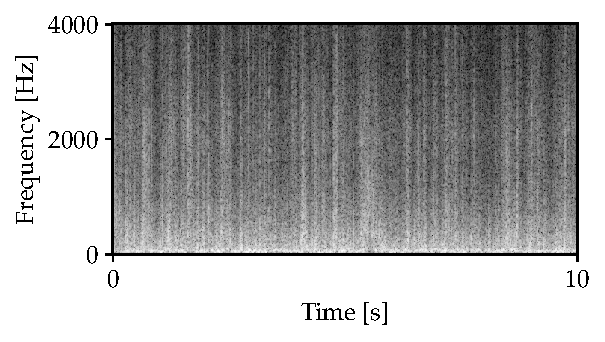
\includegraphics[width=\textwidth]{img/rumble.pdf}
		\subcaption{}
	\end{subfigure}	
	\begin{subfigure}[b]{0.45\columnwidth}
		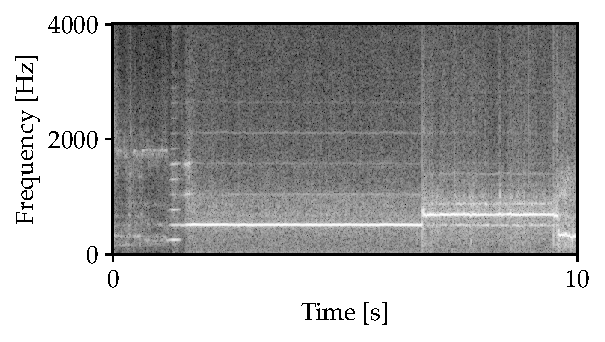
\includegraphics[width=\textwidth]{img/whistle.pdf}
		\subcaption{}
	\end{subfigure}
	
	
	\caption[SampleRNN - Raw Audio Generation]{Spectrograms of several classes of outputs from sampleRNN: choir textures (a), speech-like babbling (b), rumble (c), whistle (d). The choir textures are obtained from the Chorales training set, while the others are from the Rima Glottidis training set. The main two tones in Figure (d) are a C5 and a F5.}
	\label{fig:esempi}
\end{figure}


%%%%%%%%%%%%%%%%%%%%%%%%%%%%%%%%%%%%%%%%%%%%%%%%%%%%%%%%%%%
% Back matter contents
%%%%%%%%%%%%%%%%%%%%%%%%%%%%%%%%%%%%%%%%%%%%%%%%%%%%%%%%%%%
\backmatter

\cleardoublepage
\phantomsection
\addcontentsline{toc}{chapter}{List of Publications}
\chapter*{List of Publications}
\pagestyle{plain}
%\chaptermark{ }
%\sectionmark{ }
%\addcontentsline{toc}{chapter}{List of Publications}

\newcounter{pubs_counter}

\begin{list}{[\arabic{pubs_counter}]~}{\usecounter{pubs_counter}}

\item
E.~Marchi, F.~Vesperini, S.~Squartini, and B.~Schuller, ``Deep recurrent neural network-based autoencoders for acoustic novelty detection,'' \emph{Computational Intelligence and Neuroscience}, 2016.

\item
F.~Vesperini, P.~Vecchiotti, E.~Principi, S.~Squartini, and F.~Piazza, ``Localizing speakers in multiple rooms by using deep neural,'' \emph{Computer Speech and Language}, 2017.

\item
F.~Vesperini, L.~Gabrielli, E.~Principi, and S.~Squartini,``Polyphonic sound event detection by using capsule neural networks,'' \emph{Journal of Selected Topics in Signal Processing}, 2018, submitted.

\item
E.~Marchi, F.~Vesperini, F.~Eyben, S.~Squartini, and B.~Schuller, ``A Novel Approach for Automatic Acoustic Novelty Detection Using a Denoising Autoencoder with Bidirectional LSTM Neural Networks,'' \emph{Proc. of ICASSP}, Brisbane, Australia, 19-24 Apr. 2015, IEEE.

\item
E.~Marchi, F.~Vesperini, F.~Weninger, F.~Eyben, S.~Squartini, and B.~Schuller, ``Non-Linear Prediction with LSTM Recurrent Neural Networks for Acoustic Novelty Detection,'' \emph{Proc. of IJCNN}, Killarney, Ireland, 12-16 Jul. 2015, IEEE.

\item
F.~Vesperini, P.~Vecchiotti, E.~Principi, S.~Squartini, and F.~Piazza, ``Deep neural networks for multi-room voice activity detection: Advancements and comparative evaluation,'' \emph{Proc. of IJCNN}, Vancouver, Canada, 24-29 Jul. 2016, IEEE, pp. 3391--3398.

\item
M.~Gasparini, F.~Vesperini, S.~Cecchi, S.~Squartini, F.~Piazza, and R.~Toppi, ``Combining evolution strategies and neural network procedures for compression driver design,'' \emph{Proc. of IJCNN}, Vancouver, Canada, 24-29 Jul. 2016, IEEE, pp. 3385--3390.

\item
P.~Vecchiotti, F.~Vesperini, E.~Principi, S.~Squartini, and F.~Piazza, ``Convolutional neural networks with 3-{D} kernels for voice activity detection in a multiroom environment,'' \emph{Multidisciplinary Approaches to Neural Computing}, pp. 161--170. Springer, 2018.

\item
F.~Vesperini, P.~Vecchiotti, E.~Principi, S.~Squartini, and F.~Piazza, ``A neural network based algorithm for speaker localization in a multi-room environment,'' \emph{Machine Learning for Signal Processing (MLSP), 2016 IEEE 26th International Workshop on}. IEEE, 2016, pp. 1--6.

\item
E.~Principi, F.~Vesperini, S.~Squartini, and F.~Piazza, ``Acoustic novelty detection with adversarial autoencoders,'' \emph{Proc. of IJCNN}, Anchorage, Alaska, 14-19 May 2017, IEEE, pp. 3324--3330.

\item
M.~Valenti, D.~Tonelli, F.~Vesperini, E.~Principi, and S.~Squartini, ``A neural network approach for sound event detection in real life audio,'' \emph{Proc. of EUSIPCO}, Kos, Greece, Sept. 2017, IEEE.

\item
L.~Gabrielli, C.~E. Cella, F.~Vesperini, D.~Droghini, E.~Principi, and S.~Squartini, ``Deep learning for timbre modification and transfer: An evaluation study,'' \emph{Proc. of 144th AES}, Milan, Italy, 24-26 May 2018, Audio Engineering Society.

\item
L.~Ambrosini, L.~Gabrielli, F.~Vesperini, S.~Squartini, and L.~Cattani, ``Deep neural networks for road surface roughness classification from acoustic signals,'' \emph{Proc. of 144th AES}, Milan, Italy, 24-26 May 2018, Audio Engineering Society.

\item
F.~Vesperini, A.~Galli, L.~Gabrielli, E.~Principi, and S.~Squartini, ``Snore sounds excitation localization by using scattering transform and deep neural networks,'' \emph{Proc. of IJCNN}, Rio de Janeiro, Brasil, 8-13 Jul. 2018, IEEE.

\item
F.~Vesperini, D.~Droghini, E.~Principi, L.~Gabrielli, and S.~Squartini, ``Hierarchic {C}onv{N}ets framework for rare sound event detection,'' \emph{Proc. of EUSIPCO}. IEEE, Sept. 3-7 2018.

\item
F.~Vesperini, L.~Romeo, E.~Principi, A.~Monteri\`{u}, and S.~Squartini, ``Convolutional recurrent neural networks and acoustic data augmentation for snore detection,'' \emph{Proc. of WIRN}, Vietri sul Mare, Italy, 13-15 Jun. 2018.

\item
D.~Droghini, F.~Vesperini, E.~Principi, S.~Squartini, and F.~Piazza, ``Few-shot siamese neural networks employing audio features for human-fall detection,'' \emph{Proc. of The International Conference on Pattern Recognition and Artificial Intelligence}, Union, NJ, USA, Aug. 15-17 2018.

  
\end{list}
\newpage
\textbf{Others}:
\begin{list}{[\arabic{pubs_counter}]~}{\usecounter{pubs_counter}}
\item
F.~Vesperini, D.~Droghini, D.~Ferretti, E.~Principi, L.~Gabrielli, S.~Squartini, and F.~Piazza, ``A hierarchic multi-scaled approach for rare sound event detection,'' Ancona, Italy, 2017, {DCASE} {T}ech. {R}eport. {C}opyright-free.

\item 
F.~Vesperini, L.~Gabrielli, E.~Principi, and S.~Squartini, ``A capsule neural networks based approach for bird audio detection,'' Ancona, Italy, 2018, {DCASE} {T}ech. {R}eport. {C}opyright-free.

\item
L.~Gabrielli, F.~Vesperini, D.~Droghini, and S.~Squartini, ``Rima {G}lottidis: Experimenting generative raw audio synthesis for a sound installation,'' \emph{XXII Colloquium of Musical Informatics}, Udine, Italy, 20-23 Nov. 2018.

\end{list}
	





\bibliographystyle{IEEEbib}
\bibliography{IEEEabrv,refs}

\end{document}
